\documentclass{article}

\usepackage[dblblindworkshop]{neurips_2026}
\workshoptitle{Economics for Machine Learning}
% The bundled 2026 style's anonymous notice branch otherwise ignores the
% workshop track name and prints the regular main-conference submission footer.
\makeatletter
\renewcommand{\@noticestring}{\@trackname}
\makeatother

\usepackage[utf8]{inputenc}
\usepackage[T1]{fontenc}
\usepackage{hyperref}
\usepackage{url}
\usepackage{booktabs}
\usepackage{amsmath,amsfonts,amssymb}
\usepackage{microtype}
\usepackage{xcolor}
\usepackage{graphicx}
\usepackage{subcaption}
\usepackage{multirow}
\usepackage{tabularx}
\usepackage{siunitx}
\usepackage{float}
\usepackage{placeins}
\usepackage{pgfplots}
\pgfplotsset{compat=1.18}
\sisetup{detect-all,table-number-alignment=center}
\hypersetup{colorlinks=true,linkcolor=blue!55!black,citecolor=blue!55!black,urlcolor=blue!55!black}

\title{Reasoning Compute as a Strategic Input:\\Auction-Grounded Frontiers in a Parametric Contest}

\author{Anonymous Author(s)}

\begin{document}
\maketitle

\begin{abstract}
Economic evaluation of reasoning compute must distinguish better decisions from stronger incentives to win business. We measure held-out bidder utility for six language-model checkpoints on 216 auction decision tasks under externally assigned, fixed-length reasoning budgets. Increasing the budget from 0 to 768 tokens improves endpoint performance under both utility-ratio and dollar-profit aggregation, although intermediate gains are uneven and a calculator outperforms every fixed-budget model. We then use the measured compute--quality curves in a specified contest between decision-service providers, separating contract selection and client benefit from auction winning and surplus. The contest's incentives generate overcompute, alignment, and undercompute; the measurements determine transition locations and allocation consequences. Complete equilibrium analysis and quality-mapping sensitivity clarify these conditional predictions. At the illustrative monetary benchmark, private and planner allocations both reach the tested budget ceiling. The resulting contribution is an economic measurement framework with explicit strategic assumptions: improved decision utility can justify additional compute without establishing that competition causes excessive expenditure.
\end{abstract}

\section{Introduction}
\label{sec:introduction}

Inference compute is a costly input to automated decisions: additional reasoning tokens can improve an action without changing model parameters \citep{snell2024scaling,wu2024inference,alomrani2025budget}. A decision maker weighs the gain against its cost. Competition adds a second return when improved quality helps a provider win business, so privately attractive compute need not maximize user value net of all providers' costs.

Consider two providers competing for one fixed-payment decision-service contract. Each chooses an inference budget and pays its compute cost; a client selects a provider using demonstrated quality and benefits from the winner's output. This motivates our contest. Auction decisions supply a benchmark for service quality, while the contract supplies the modeled prize.

We measure held-out bidder utility for six checkpoints on 216 constructed auction tasks. Models receive private values, feasible bids and estimated win probabilities, then select a bid under an assigned token budget. Utility ratio, dollar profit and regret distinguish the consequences of errors that accuracy treats alike. Supplied probabilities make this a controlled calculation and action-selection task, with a construction-split calculator as a practical reference.

We insert the measured curves into a specified service contest. Contract selection and client benefit are assumed mappings, distinct from auction winning and total surplus. Three allocation regions are structural; measurements contribute their transition locations, uncertainty and consequences. At the illustrative monetary benchmark with $\gamma=1$, both private and planner allocations reach 768 tokens per provider, the tested ceiling.

\paragraph{Contributions and takeaway.}
We contribute held-out economic-utility frontiers, a service-contest interpretation with explicit payoff and welfare accounting, and conditional private--planner boundaries with equilibrium and mapping sensitivity. The takeaway is that improved decision utility does not by itself establish excessive competitive compute. Code and preserved outputs are available in the reproducibility repository.\footnote{\url{https://anonymous.4open.science/r/reasoning-compute-economic-utility-EED7/}}

\section{Related work}

Test-time scaling studies compare resource allocations across prompts, sampling and search procedures \citep{wei2022chain,snell2024scaling,wu2024inference,alomrani2025budget,hariri2026scaling}. \citet{wan2026shadowprice} study centralized allocation under a token constraint; our question concerns decentralized incentives. Confidence-based stopping and sampling address a different uncertainty tradeoff \citep{jurayj2025finalanswer,shi2025reasoninguncertainty,xie2026statistical}.

Economic benchmarks evaluate rational choice, bargaining and market interaction \citep{raman2024steer,raman2025steerme,fish2025econevals,chen2024aucarena,zhu2024synthetic,deng2024bargaining}. Bazaar studies repeated pricing with hidden preferences and provider-specific effort settings \citep{ahmed2026bazaar}. Our task instead controls generated trace length and scores bidder utility on held-out prices; option-order sensitivity motivates randomized presentation and a common readout \citep{pezeshkpour2024order}.

Our service contest draws on rent-seeking theory \citep{tullock1980efficient} and provider competition over compute \citep{artola2026games}. The latter evaluates math and science benchmark performance, whereas we use held-out auction utility and propagate scenario and generation uncertainty. Our distinction is the economic measurement entering conditional allocation boundaries, not a new competitive mechanism. Appendix Table~\ref{tab:related_work_positioning} gives the detailed comparison, and Figure~\ref{fig:pipelineoverview} summarizes the measurement-to-model pipeline.

\section{Economic framework}

\subsection{Auction decision problem}

In the empirical task, a bidder model is supplied with private value $v$ and selects a bid $b\leq v$ from the candidate set. We approximate the price required to win by a random historical closing price $P$. Its empirical CDF $\widehat F_P(b)$---the share of closing prices at or below $b$---gives the estimated winning probability and expected utility
\begin{equation}
 \widehat p(b)=\widehat F_P(b)=\frac{1}{N}\sum_{n=1}^{N}\mathbf{1}\{P_n\leq b\},
 \qquad U(b\mid v)=\widehat p(b)(v-b).
 \label{eq:auctionutility}
\end{equation}
This reduced-form calculation treats an observed closing price as the price a bidder must beat and imposes risk neutrality. For scenario $s$, candidate set $B_s$, and private value $v_s$, the benchmark action is $b_s^*=\arg\max_{b\in B_s}U_s(b\mid v_s)$. Model $m$ at budget $c$ selects $\widehat b_{msc}$. We report exact optimality, regret (foregone expected profit), and utility ratio (the share of feasible optimum captured):
\begin{equation}
 A_{msc}=\mathbf{1}\{\widehat b_{msc}=b_s^*\},\quad
 R_{msc}=U_s(b_s^*\mid v_s)-U_s(\widehat b_{msc}\mid v_s),\quad
 Q_{msc}=\frac{U_s(\widehat b_{msc}\mid v_s)}{U_s(b_s^*\mid v_s)}.
 \label{eq:metrics}
\end{equation}
The denominator is positive in every constructed scenario, so $Q_{msc}$ is well defined. We aggregate with equal scenario weights,
\begin{equation}
 q_m(c)=\frac{1}{S}\sum_{s=1}^{S}Q_{msc},\qquad
 \overline R_m(c)=\frac{1}{S}\sum_{s=1}^{S}R_{msc},\qquad
 \overline A_m(c)=\frac{1}{S}\sum_{s=1}^{S}A_{msc}.
 \label{eq:frontier}
\end{equation}
Our primary outcome, $q_m(c)$, distinguishes the profit consequences of choices that exact accuracy counts equally: missing an optimum by one dollar and by one hundred dollars are both errors, but have different economic losses. We also report mean dollar-valued expected bidder profit, $\overline U_m(c)=S^{-1}\sum_s U_s(\widehat b_{msc}\mid v_s)$, and regret. The mean scenario utility ratio gives each scenario equal weight in normalized units; mean profit gives each dollar equal weight across the constructed scenarios. These objectives need not rank budgets identically, and neither is total auction surplus. Repeated generations or option orders are averaged first within each scenario--budget cell. Treating reasoning tokens as a manipulable decision resource yields the measured, discrete frontier $\{q_m(c):c\in\mathcal C\}$, which enters the analysis in its observed form without smoothing or a monotonicity restriction.

\subsection{Strategic reasoning-compute game}

\paragraph{Participants, contract, and benchmark quality.}
Two symmetric providers choose budgets $c_i\in\mathcal C$ before competing for one service contract. Each incurs its inference cost; the winner receives client payment $V$. Measured auction utility ratio $q(c_i)$ is the service-quality proxy. We assume, rather than estimate, that this quality determines contract selection and that client benefit is linear in selected quality:
\begin{equation}
 P_i(c_i,c_j;\gamma)=\frac{q(c_i)^\gamma}{q(c_i)^\gamma+q(c_j)^\gamma},\qquad
 \pi_i(c_i,c_j)=V P_i(c_i,c_j;\gamma)-\lambda c_i.
 \label{eq:contest}
\end{equation}
Here $V>0$ is the private prize, $\lambda$ is per-token cost, and $\gamma$ governs how strongly quality affects winning: near zero it approaches an even split, while larger values favor the higher-quality agent. Dividing by $V$ yields
\begin{equation}
 \widetilde\pi_i=P_i(c_i,c_j;\gamma)-\underbrace{\frac{\lambda}{V}}_{\kappa}c_i,
 \qquad \boxed{\kappa=\lambda/V},
 \label{eq:normalizedprivate}
\end{equation}
so private choice depends on cost relative to payment. Contract selection $P_i$ differs from the auction probability $\widehat p(b)$ used to score bids: better shading can raise bidder profit without increasing auction wins.

The absolute utility ratio has a task-specific origin: zero captures none of the feasible optimum and one captures all of it. Its cardinal contest interpretation remains an assumption. Common positive rescaling cancels from the Tullock rule; an origin shift changes incentives (Section~\ref{sec:strategicresults}).

A symmetric pure equilibrium is a mutual best response over the menu. Compute choices are solved in the specified game; the evaluated LLMs do not choose budgets.

\paragraph{Planner objective and its scope.}
The client obtains modeled service benefit $\beta q(c_{\mathrm{winner}})$, where $\beta>0$ converts benchmark quality into value. Summing the client's benefit net of payment with the providers' payoffs cancels the fixed contract payment $V$. The planner's objective is consequently selected-service benefit net of both providers' compute costs:
\begin{equation}
 W_{\beta}(c_1,c_2)=\beta Q_\gamma(c_1,c_2)-\lambda(c_1+c_2),
 \quad Q_\gamma=P_1q(c_1)+P_2q(c_2).
\label{eq:welfare}
\end{equation}
Here $P_1$ and $P_2=1-P_1$ allocate the service contract. This is modeled service welfare, distinct from auction total surplus. Historical prices do not identify the service payment or client value. Dividing by $V$ gives
\begin{equation}
 \widetilde W=\underbrace{\frac{\beta}{V}}_{\rho}Q_\gamma(c_1,c_2)
 -\kappa(c_1+c_2),\qquad \boxed{\rho=\beta/V}.
 \label{eq:normalizedwelfare}
\end{equation}
Thus every equilibrium and planner allocation is determined by $(\kappa,\rho,\gamma)$; only their ratios matter for the normalized game. Let $c_{\mathrm{NE}}$ be the lowest-budget symmetric mutual best response under exact ties, and let $(c_1^*,c_2^*)$ maximize Eq.~\eqref{eq:normalizedwelfare}. Define $C_{\mathrm{NE}}=2c_{\mathrm{NE}}$ and $C_{\mathrm{OPT}}=c_1^*+c_2^*$. We classify each parameter point as overcompute, aligned, or undercompute according as $C_{\mathrm{NE}}$ is greater than, equal to, or less than $C_{\mathrm{OPT}}$.

We retain the price of reasoning competition (PoRC), $C_{\mathrm{NE}}/C_{\mathrm{OPT}}$, as a menu-dependent compute ratio. On $\{128,384,768\}$, its largest possible value is $1536/256=6$; attaining six therefore reaches the menu's arithmetic ceiling rather than estimating an unrestricted inefficiency bound. We use normalized absolute welfare loss $\Delta\widetilde W=\widetilde W_{\mathrm{OPT}}-\widetilde W_{\mathrm{NE}}=\Delta W/V$. The appendix preserves the supplementary relative-loss statistic and its fixed near-zero omission rule, which plays no role in defining phase regions.

The discrete thresholds make the comparative statics explicit. Against fixed $c_j$, a unilateral increase $c_a\to c_b$ is privately profitable when
\begin{equation}
 \kappa<\frac{P_i(c_b,c_j;\gamma)-P_i(c_a,c_j;\gamma)}{c_b-c_a}.
 \label{eq:privatethreshold}
\end{equation}
For two planner allocations differing by $(\Delta Q_\gamma,\Delta C)$, the higher-compute allocation is preferred when
\begin{equation}
 \frac{\kappa}{\rho}=\frac{\lambda}{\beta}<\frac{\Delta Q_\gamma}{\Delta C}.
 \label{eq:plannerthreshold}
\end{equation}
Appendix~\ref{app:completeequilibria} characterizes the full finite-game equilibrium set, resolving mixed strategies and boundary multiplicity beyond the symmetric-pure phase plots.

\section{Empirical methodology and experimental setup}

\subsection{Dataset and tasks}

We use the Online Auctions Dataset distributed with \citet{jank2010modeling}, containing 10,681 bid records from 628 eBay auctions \citep{onlineauctionsdataset}. The evaluation covers Palm Pilot M515 PDA, Xbox game console, and Cartier wristwatch auctions. Within each category, auctions with internally inconsistent opening bids are removed and the remaining auctions are deterministically assigned, using seed 20260819, to a 70\% construction split and a 30\% held-out scoring split. The construction split determines the displayed empirical win probabilities and task support; the held-out split is used only to score decisions. Historical closing prices provide the reduced-form price-to-beat proxy used in the utility calculation.

For each category, 18 private values are selected from a five-dollar grid spanning the central-to-upper range of the construction-price distribution. At every value, we generate two independently seeded candidate sets for each option-set width $K\in\{5,7\}$, yielding $3\times18\times2\times2=216$ scenarios. Candidate bids come from feasible five-dollar grid points, sampled either through a randomly located contiguous window or as an unstructured set. Because this generation step is independent of the train- and test-optimal bids, the utility-maximizing option can occupy any identity or sorted position.

The prompt provides the private value, candidate bids, and construction-sample win probabilities; the model must calculate $(v-b)\widehat p_{\mathrm{construction}}(b)$, the utility in Eq.~\eqref{eq:auctionutility} evaluated on the construction split. Primary regret, exact optimality, and utility ratio instead use $\widehat p_{\mathrm{heldout}}(b)$, rewarding choices that transfer beyond the displayed sample. Greedy evaluation repeats each scenario under option-order seeds $\{11,23,37\}$. Every record stores the order, and scoring follows candidate labels rather than displayed positions.

The unit of observation is a scenario--checkpoint--budget--replication cell, with the underlying scenario fixed across budgets. Repeated option orders separate presentation from the decoding variation in stochastic generations. Reference policies are a construction-split calculator, uniform random choice, median displayed position, highest win probability, and a held-out oracle; the median diagnoses positional preference.

\subsection{Models and reasoning protocol}

We evaluate Phi-mini, Qwen3-4B, DeepSeek-8B, Qwen3-8B, Qwen3-14B, and Granite-8B \citep{microsoft2025phireasoning,yang2025qwen3,guo2025deepseek,ibmgranite2025}; full repository IDs and environment details appear in Appendix~\ref{app:reproducibility}.

We use $\mathcal C_G=\{0,64,128,256,512,768\}$ for the greedy frontier and $\mathcal C_S=\{128,384,768\}$ for the stochastic frontier. The common constrained option-letter readout defines the primary action; a separate free-form answer is retained for audit. Positive budgets force exactly $c$ generated trace tokens by matching minimum and maximum lengths and suppressing end-of-sequence stopping. Zero skips trace generation, and answer-stage tokens are excluded. Thus the intervention is assigned trace length, not natural reasoning completion. Table~\ref{tab:protocolmap} lists the budgets, decoding and replications; Appendix~\ref{app:computationalprotocol} provides implementation details.

Granite exposes a \texttt{thinking=True} chat-template argument rather than Qwen's native \texttt{enable\_thinking} interface. Its externally budgeted intermediate generation, constrained readout, and scoring are otherwise identical; we therefore treat Granite as a cross-family protocol sensitivity rather than a protocol-identical replication.

The stochastic frontier fixes presentation order at seed 314159 and varies generation seeds. The runner records tokens, runtime, NVML energy and memory, confidence, and both readouts. Section~\ref{sec:monetarybenchmark} applies documented rental-price assumptions to saved runtime measurements.

Table~\ref{tab:protocolmap} summarizes the protocol behind each result. The greedy and stochastic frontiers use different decoding and presentation replications and are kept separate; only the declared hybrid sensitivity combines them.
\begin{table}[htbp]
\centering\footnotesize
\caption{Which inference protocol supports each result. Positive fixed budgets force generated trace length; both answer readouts are separate stages. All primary historical decisions are scored on the held-out CDF.}
\label{tab:protocolmap}
\setlength{\tabcolsep}{4pt}
\begin{tabularx}{\linewidth}{@{}p{0.15\linewidth}p{0.25\linewidth}p{0.20\linewidth}X@{}}
\toprule
Analysis & Budgets and decoding & Replications / readout & Result and scope \\
\midrule
Greedy frontier & $0,64,128,256,512,768$; deterministic & Three option orders; constrained letter & Primary 0-to-768 utility, accuracy and profit comparisons; fixed-length intervention. \\
Stochastic frontier & $128,384,768$; $T=0.6$, top-$p=0.95$ & Five generation seeds; one fixed order; constrained letter & Generation uncertainty and primary three-budget contest inputs. \\
Free-form audit & Same stored greedy traces & Up to 20 answer tokens; exact candidate-bid parser & Agreement and paired valid-endpoint sensitivity; invalid responses remain missing. \\
Controls & No-thinking; unconstrained up to 1,024 tokens & Three option orders; constrained letter & Reference performance; excluded from primary games. Native thinking flag depends on template support. \\
Hybrid game & Deterministic zero plus stochastic $128,384,768$ & Zero averaged over orders; positives sampled jointly by seed & Zero-action sensitivity; combines protocols rather than extending a matched stochastic frontier. \\
Synthetic IPV & $0,64,128,256,$\newline $384,512,768$; deterministic & Three option orders; constrained letter & Exact-payoff robustness under specified independent opponents; a separate environment. \\
\bottomrule
\end{tabularx}
\end{table}


\subsection{Game computation}
\label{sec:gamecomputation}

We insert each stochastic frontier on $\mathcal C_S=\{128,384,768\}$ into Eqs.~\eqref{eq:normalizedprivate}--\eqref{eq:normalizedwelfare}, without smoothing. All ordered pairs are enumerated for the planner and representative symmetric-pure plots, with lowest-budget tie breaking. The full equilibrium set is computed separately (Appendix~\ref{app:completeequilibria}). The primary game excludes controls; Appendix~\ref{app:zeroaugmented} combines deterministic zero with stochastic positive budgets as a protocol-mixed sensitivity.

The phase analysis maps $\kappa\in[5\times10^{-9},1.2\times10^{-3}]$ and $\rho\in[10^{-3},40]$ on 181 log-spaced points per axis for $\gamma\in\{0.5,1,2,4\}$. The lower $\kappa$ bound includes the monetary benchmark in Section~\ref{sec:monetarybenchmark}; the remaining extent follows earlier parameter sweeps. This grid is only a rendering device: it carries no probability weights, and shaded areas are not likelihoods. Separately, we compute every exact payoff-indifference value in Eqs.~\eqref{eq:privatethreshold}--\eqref{eq:plannerthreshold} and verify the allocations on either side.

Appendix~\ref{app:strategicrobustness} retains supplementary raw-grid and deterministic-menu sensitivity checks; the latter changes both the menu and decoding frontier.

\subsection{Uncertainty quantification}
\label{sec:uncertainty}

We preserve cross-budget dependence in each bootstrap. For a paired scenario draw $d$, the same sampled indices are applied at every budget:
\begin{equation}
 q_m^{(d)}(c)=\frac{1}{S}\sum_{r=1}^{S}Q_{m,I_r^{(d)},c}.
 \label{eq:bootstrapfrontier}
\end{equation}
For greedy endpoints and log-budget slopes, orders are averaged within scenario--budget cells before 2,000 paired scenario draws. The supplementary profit analysis resamples 54 product/private-value families within the three fixed products, retaining each family's four candidate variants and complete budget vector, in 10,000 draws (seed 20261006). Table~\ref{tab:familyendpoints} reports pointwise 95\% intervals.

The stochastic bootstrap samples scenarios and one stored generation seed jointly across budgets in 1,000 draws. The hybrid game uses the same procedure with order-averaged zero added. Separately, 2,000 within-product auction draws resample held-out prices and re-score fixed choices, isolating CDF estimation uncertainty. All intervals condition on original prompts, products and construction split; prompt-side changes require new inference. Appendix~\ref{app:prospectiveuq} gives the detailed protocols.

\subsection{Free-form readout sensitivity}
\label{sec:freeformmethod}

Free-form bids are valid only when the fixed parser returns a displayed candidate. Endpoint sensitivity retains scenario--order cells valid at both 0 and 768, averages paired differences within scenario, and uses 2,000 paired scenario draws. Invalid responses remain missing; changing validity therefore changes sample composition.

\section{Results}
\FloatBarrier

\subsection{Leakage-controlled deterministic scaling}

Figure~\ref{fig:quality} and Table~\ref{tab:crossmodel} summarize the order-averaged greedy frontier over all 216 scenarios. The 0-to-768 gain ranges from 0.111 for Phi-mini to 0.175 for DeepSeek-8B; Granite-8B gains 0.157 [0.122, 0.190]. All six paired intervals exclude zero; none of the 2,000 draws crosses zero. At 768 tokens, utility ratios range from 0.829 to 0.950 and exact optimality from 38.3\% to 64.7\%. Every constrained output is valid.

The adjacent-budget pattern is less tidy. DeepSeek-8B falls between 0 and 64 tokens, Qwen3-4B falls at 128, Granite-8B falls slightly at 256, and several intermediate increments are small; much of the improvement arrives after 512 tokens. Even so, the regression slope of utility ratio on log budget over the five positive budgets is positive for every checkpoint, ranging from 0.0117 to Granite-8B's 0.0191 [0.0154, 0.0231].

\begin{figure}[H]
\centering
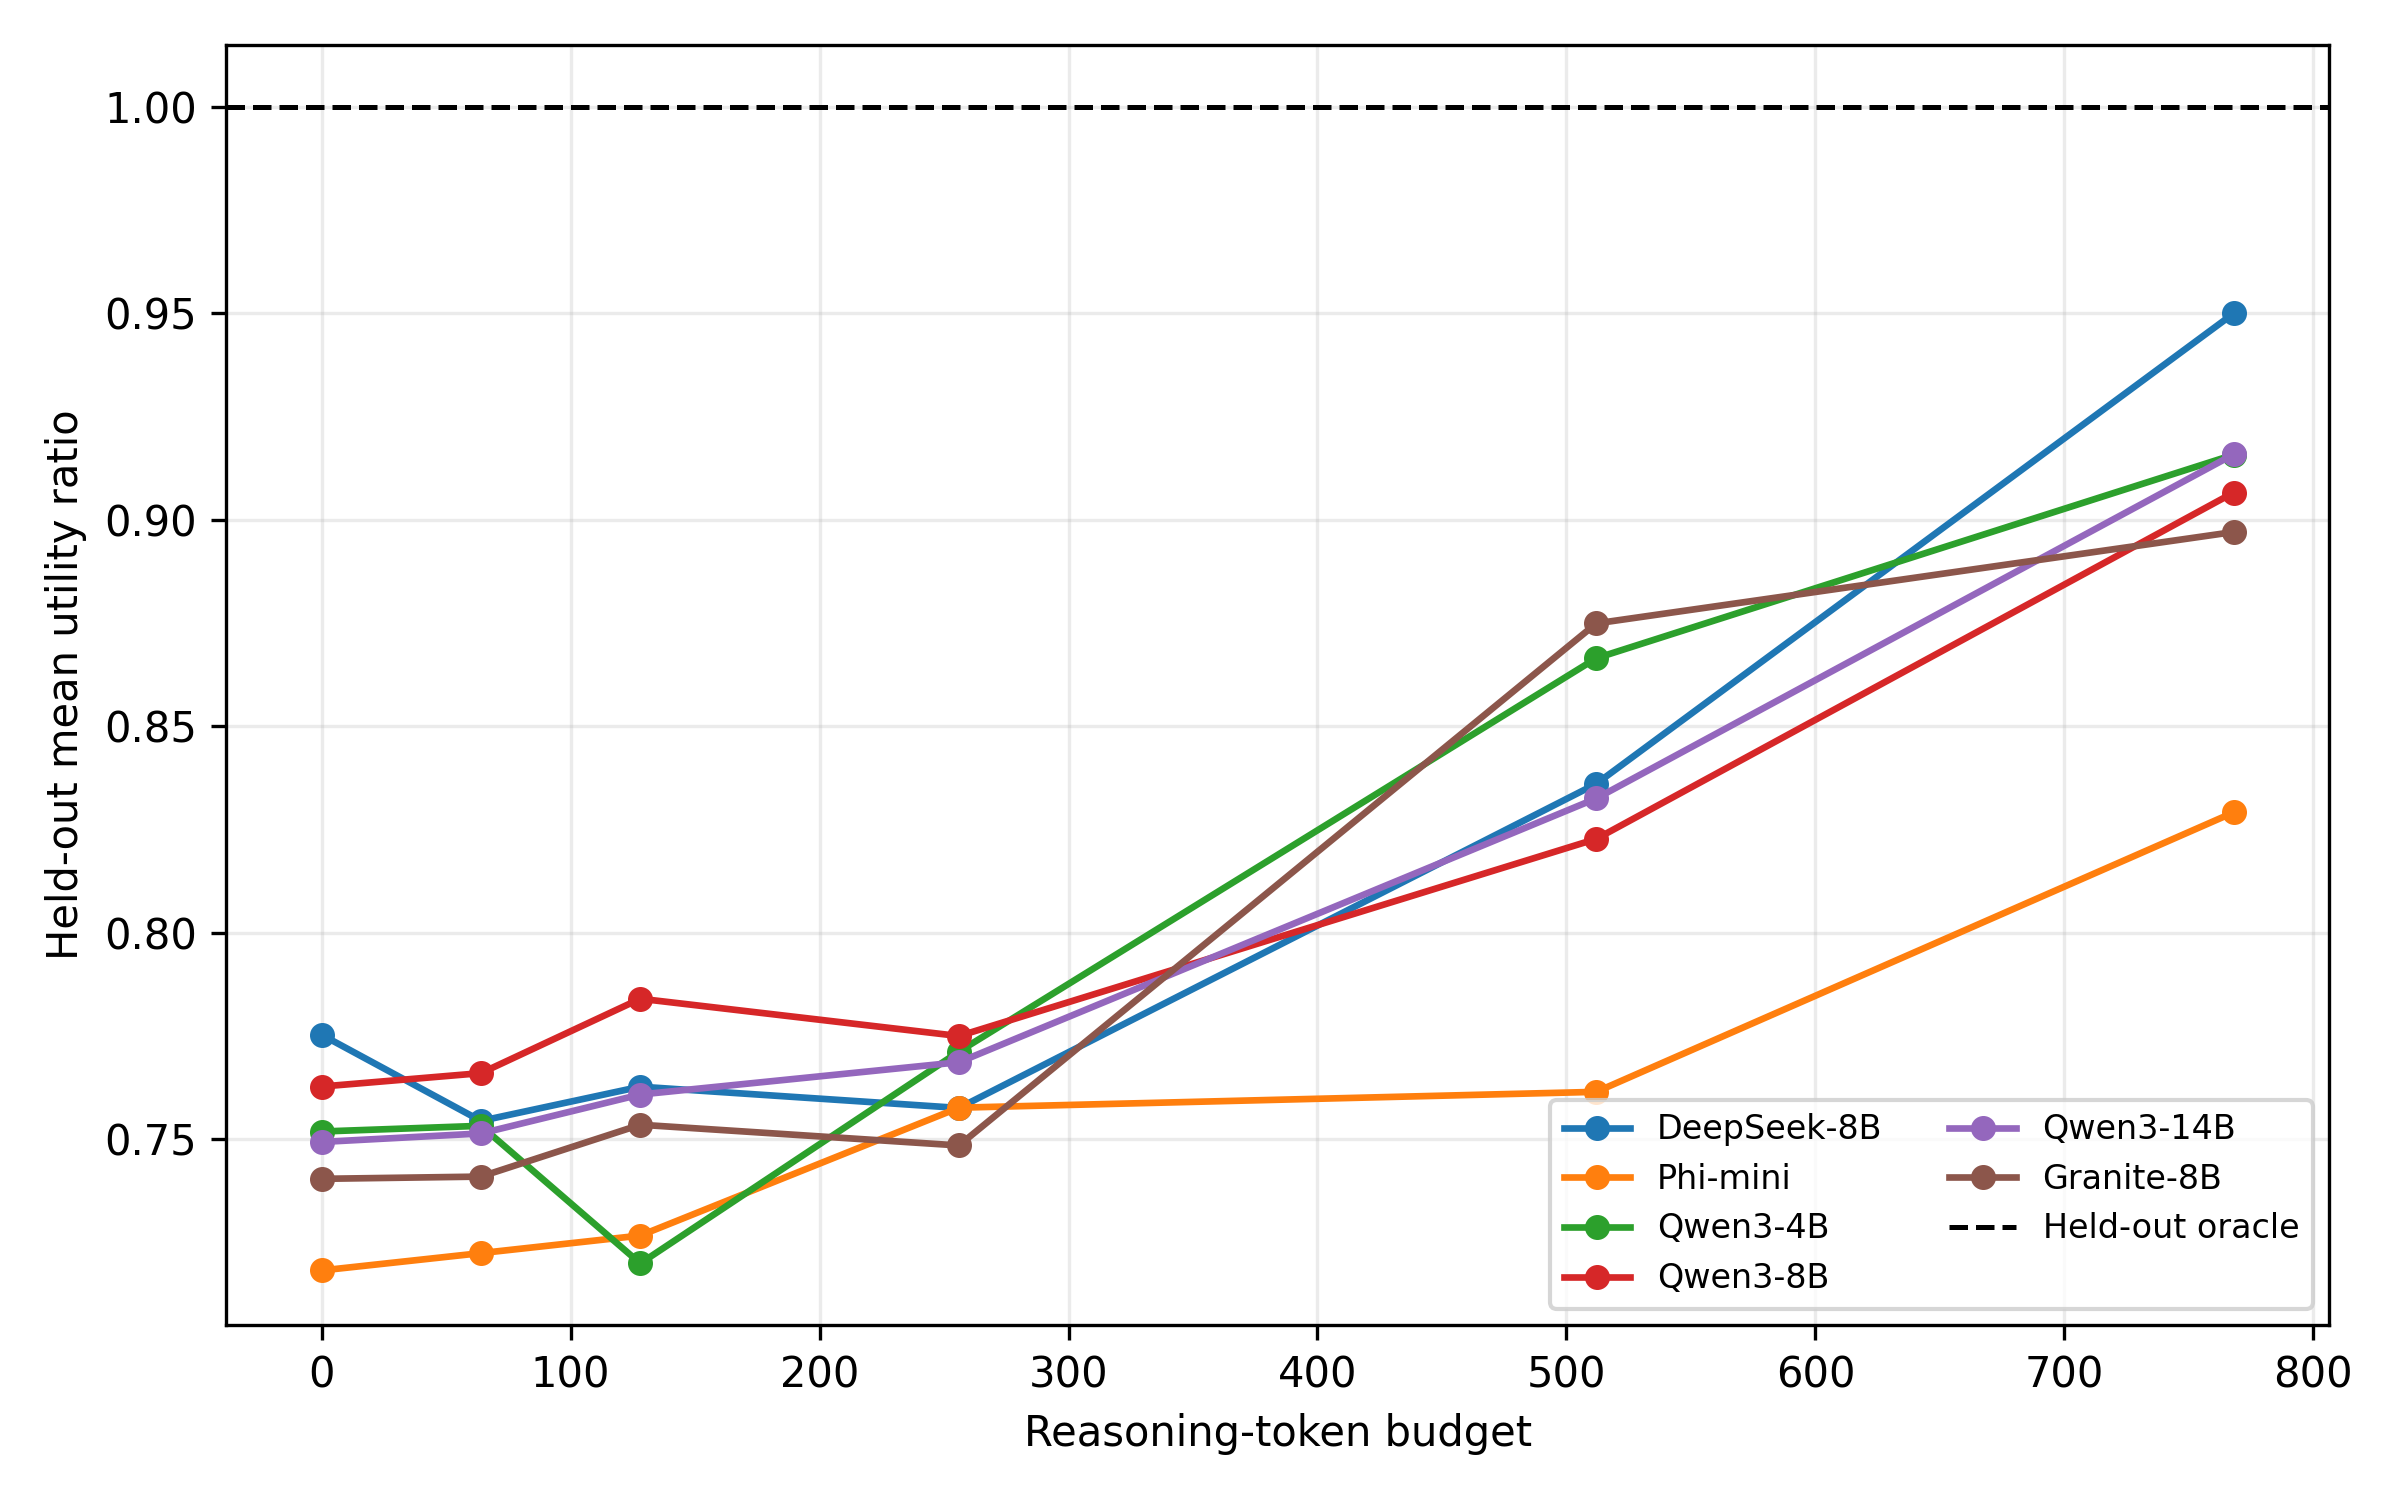
\includegraphics[width=0.93\linewidth]{figures/leakage_free_compute_quality.png}
\caption{Held-out compute--utility frontiers, averaging 216 scenarios and three option orders per scenario. Lines connect evaluated greedy budgets and do not impose monotonicity; the dashed line is the held-out oracle.}
\label{fig:quality}
\end{figure}

\begin{table}[H]
\centering
\caption{Order-averaged deterministic endpoints over 216 paired scenarios. Accuracy is percent; intervals are 95\% paired scenario-bootstrap intervals for $q(768)-q(0)$.}
\label{tab:crossmodel}
\small
\setlength{\tabcolsep}{3.5pt}
\begin{tabular}{lrrrrr}
\toprule
Model & $q(0)$ & $q(768)$ & Difference (95\% CI) & Acc. 0 & Acc. 768 \\
\midrule
DeepSeek-8B & 0.775 & 0.950 & 0.175 [0.147, 0.204] & 21.5 & 64.7 \\
Phi-mini & 0.718 & 0.829 & 0.111 [0.085, 0.139] & 19.1 & 38.3 \\
Qwen3-4B & 0.752 & 0.916 & 0.164 [0.136, 0.193] & 21.1 & 57.4 \\
Qwen3-8B & 0.763 & 0.907 & 0.144 [0.118, 0.170] & 23.1 & 55.2 \\
\bottomrule
\end{tabular}
\end{table}


\subsection{Economic magnitude and aggregation sensitivity}

The supplementary family-clustered analysis preserves positive 0-to-768 gains under both mean scenario utility ratio and mean dollar-profit aggregation for all six checkpoints (Appendix Table~\ref{tab:familyendpoints}). Expected bidder-profit gains range from \$11.11 to \$46.36 per constructed decision, with all pointwise 95\% family intervals excluding zero. These dollar amounts quantify the consequences of the chosen bids under the reduced-form held-out scoring environment; they are neither observed realized earnings nor changes in total auction surplus.

Aggregation matters more for intermediate comparisons. Nine of the 30 adjacent-budget comparisons have opposite point directions under ratio and dollar-profit aggregation, but none supports both opposite directions under the family-clustered intervals. We therefore do not claim a statistically established ranking reversal. The contribution of economic scoring is to expose error magnitude and the objective's weighting, rather than to guarantee a different preferred budget from accuracy or from another utility metric.

\subsection{Baselines and task breadth}

The median-position policy achieves 0.725 utility ratio and 18.7\% accuracy. At 768 tokens, all checkpoints exceed it, random choice (0.711) and the highest-win-probability rule (0.731), but the calculator remains stronger at 0.981. A saved-decision audit also finds model-minus-calculator dollar-profit gaps of $-\$36.00$ to $-\$15.09$, with all six simultaneous exploratory bands below zero (Appendix Table~\ref{tab:calculatorerroraudit}). Unconstrained generations reach 0.846--0.972 (Table~\ref{tab:baselines}). Supplied probabilities make this a calculation and action-selection benchmark; extra LLM tokens improve the pipeline without establishing an advantage over numerical optimization. Calculator resource costs were not measured, so no deployment cost-effectiveness ranking is claimed.

\subsection{Free-form readout sensitivity}

Free-form validity is 29.1--96.7\% across checkpoints, and constrained--free-form agreement among valid responses is 32.7--82.2\% (Appendix Tables~\ref{tab:freeformsensitivity}--\ref{tab:freeformbybudget}). The five estimable paired endpoint increases are 0.161--0.230 and exclude zero. Granite-8B has no paired endpoint because none of its budget-zero free-form responses pass the fixed parser; its constrained outputs remain complete.

\subsection{Generation uncertainty}

Five stochastic generations per scenario preserve the high-budget advantage: from 128 to 768 tokens, mean utility ratio rises by 0.067--0.189 across the six checkpoints, including 0.747 to 0.886 for Granite-8B. Repeated sampling still leaves a local reversal for Phi-mini, from 0.746 at 128 to 0.744 at 384 tokens. Appendix Table~\ref{tab:stochasticfrontier} reports the hierarchical intervals.

The held-out auction-CDF bootstrap also preserves the deterministic endpoint direction for every checkpoint; Granite-8B's re-scored increase is 0.152 [0.132, 0.168]. Appendix Table~\ref{tab:auctioncdf} gives the full panel. Because prompts and choices stay fixed, these intervals isolate held-out CDF uncertainty from the scenario and generation bootstraps.

\paragraph{Synthetic robustness.}
An exact-payoff independent-private-values (IPV) benchmark changes the economic environment while retaining 216 scenarios, both candidate-set widths, and the same order seeds. Its six endpoint gains range from 0.164 to 0.288, and every paired interval excludes zero (Appendix~\ref{app:syntheticipv}); Granite-8B gains 0.217 [0.176, 0.259]. The exercise is deliberately stylized, but the same endpoint pattern appears when utility is computed without a historical closing-price CDF.

\subsection{Parametric strategic reasoning-compute results}
\label{sec:strategicresults}

At $\gamma=1$, all six frontiers yield overcompute, aligned and undercompute regions (Appendix Figure~\ref{fig:normalizedphase}). Their existence is structural under the conditions in Appendix~\ref{app:completeequilibria}; the measured contribution is the transition locations and allocation consequences. Four checkpoints move directly from 768 to 128 as $\kappa$ rises. Qwen3-4B and Granite-8B pass through 384 (Appendix Table~\ref{tab:normalizedthresholds}). Private transitions do not depend on $\rho$.

Planner compute depends on $r=\kappa/\rho=\lambda/\beta$ and moves $1536\to896\to256$ tokens as $r$ rises. The middle allocation is asymmetric: $896=768+128$, so the planner concentrates most compute on one agent. Across models, the first threshold ranges from $4.99\times10^{-5}$ to $1.31\times10^{-4}$ and the second from $5.44\times10^{-5}$ to $1.64\times10^{-4}$. These diagonal boundaries create an overcompute wedge when private incentives support high compute despite low social quality value, and an undercompute region when high $\rho$ sustains planner compute after private demand has fallen. Gray regions have equal total compute, though their underlying allocations may differ; all boundaries come from exact enumeration of the measured point frontiers.

Complete equilibrium enumeration over six point frontiers and $\gamma\in\{0.5,1,2,4\}$ finds one mixed-only open interval, for Qwen3-4B at $\gamma=4$, approximately $\kappa\in(3.28603,3.28909)\times10^{-4}$. The appendix reports its strategy, independent linear-program verification and boundary multiplicity.

At $\gamma=1$, shifting quality to $q+0.5$ reduces the private maximum-budget threshold by 36.8--39.1\% (Appendix Table~\ref{tab:qualityoriginsensitivity}). Quality increments are unchanged, but relative selection advantages change. The measurements therefore matter through their shape and level under the assumed mapping.

At $\gamma=1$, accuracy-based selection makes the threshold supporting 768/768 equal to 4.05--5.96 times its utility-based value. All six accuracy-minus-utility differences remain positive under exploratory simultaneous family/seed bootstrap bands (Appendix Table~\ref{tab:metricshapecomparison}). DeepSeek-8B's hypothetical $\kappa=1.5\times10^{-4}$ contrast---128/128 under utility versus 768/768 under accuracy---persists in all 10,000 draws. Linear interpolation has smaller point effects but uncertain shape sensitivity. Alternative profit-based and quality-difference selection rules expose further mapping dependence (Table~\ref{tab:selectionmappings}); none identifies client choice or real-market inefficiency.

Within the contest, increasing $\gamma$ strengthens private incentives for compute. Across the six frontiers, private transition thresholds move rightward as $\gamma$ rises, expanding the overcompute region (Appendix Figure~\ref{fig:normalizedphasegamma}). Increasing $\rho$ instead lowers $\kappa/\rho$, raises planner compute, and moves a point upward from overcomputation through alignment toward undercomputation.

\subsection{A monetary benchmark for relative compute cost}
\label{sec:monetarybenchmark}

Measurements already recorded by the runner supply an illustrative incremental-cost scenario for five RTX~4090 runs. OLS regressions over their stochastic records give incremental runtime of 0.0120--0.0217 seconds and GPU energy of 3.04--6.06 joules per reasoning token. Using the recorded rental-price scenario of \$0.74 per GPU-hour \citep{runpod2026pricing}, the resulting $\lambda$ estimates range from $2.46\times10^{-6}$ to $4.46\times10^{-6}$ dollars per token; Granite-8B is the upper endpoint. Qwen3-14B ran on an L40S and remains outside this hardware-matched price comparison. Valuing electricity separately at the May 2026 U.S. commercial average \citep{eia2026electricity} would double-count a cost already bundled into the rental rate.

The 189 held-out auctions have a pooled mean closing price of \$328.23. Setting the service payment $V$ to this amount supplies a normalization scenario, not an estimate of service-contract rent. The five hardware-matched estimates then imply $\kappa$ between $7.50\times10^{-9}$ and $1.36\times10^{-8}$; Granite-8B is again the upper endpoint. At $\gamma=1$, both providers' equilibrium budgets and both planner budgets equal 768 tokens throughout the plotted $\rho\in[10^{-3},40]$ range. This is alignment within the tested menu. Both allocations reach its ceiling, so the comparison cannot establish alignment beyond 768 tokens. The service payment, client valuation, and contest sensitivity remain unestimated; the rental calculation does not locate a deployed market in the phase map.

Adding the stored zero-reasoning action changes thresholds and makes zero optimal at sufficiently high cost (Appendix~\ref{app:zeroaugmented}). Raw-grid and broader deterministic-menu checks remain supplementary diagnostics; grid-area shares have no market-prevalence interpretation.

\section{Discussion}

Higher endpoint budgets capture more available bidder profit across the six checkpoints. Utility ratio and dollar profit expose error magnitude and weighting, but their endpoint agreement is stronger than the uncertain intermediate aggregation reversals. Additional LLM tokens improve this decision pipeline even though a calculator performs better. The benchmark's contribution is therefore to quantify the consequences of calculation and action-selection errors, rather than demonstrate general economic expertise.

The strategic analysis asks a separate question: how would providers purchase compute if measured quality helped them win a service contract? Competition rewards improvements in selection probability, whereas the planner values the selected service and accounts for both providers' resource costs. These incentives can disagree even with the same quality frontier. The measured curves locate where that disagreement changes allocations; the mere existence of three regions is a property of the contest. Full equilibrium handling closes the symmetric-pure restriction within the finite game, while origin sensitivity shows why a performance score alone cannot determine competitive returns. The illustrative cost benchmark yields alignment at the menu ceiling, leaving the private--planner comparison beyond that ceiling unresolved.

For the service-contract example, the useful output is a set of conditional break-even comparisons. A provider's willingness to buy additional compute depends on how clients reward quality and on the contract payment; the planner's willingness depends on the value delivered by the selected service. Changing client valuation can move the planner allocation without changing providers' incentives. This distinction explains why a compute--utility curve is necessary input to the modeled allocation question but insufficient to answer it alone. Applications require a justified selection rule and client-value mapping in addition to the measured curve and deployment-relevant costs.

\section{Limitations}

The auction tasks supply probabilities and finite candidate sets, with closing prices as an exogenous price-to-beat proxy. They do not identify rivals' values or reproduce an endogenous auction market. Three products, 216 scenarios and fixed construction/scoring splits limit generalization; bootstraps exclude market shift, prompt-side distribution changes and model misspecification.

The service contest assumes symmetric primitives, a fixed payment, Tullock selection, linear client value and a three-budget menu. Complete equilibrium analysis resolves that finite game without identifying the selection technology or client valuation. The hybrid zero-action check mixes protocols, and the monetary benchmark omits a deployment-specific cost model and remains ceiling-constrained. Modeled welfare excludes latency and environmental externalities and heterogeneous client values.

Assigned trace length does not establish completed reasoning, and tokens imperfectly proxy resources. Granite's template differs from Qwen's; original-four checkpoint revisions were recovered retrospectively under a disclosed unchanged-cache assumption (Appendix~\ref{app:reproducibility}). These restrictions bound the measurement and strategic claims.

\section{Conclusion}

Economic utility reveals the consequences of reasoning errors beyond accuracy. Higher endpoint budgets improve bidder utility in these tasks, while calculator superiority and uneven intermediate gains limit practical significance. The service contest contributes conditional allocation boundaries and exposes their dependence on selection and value assumptions. It does not establish excessive compute expenditure in deployed markets. Better decisions and efficient competition remain distinct claims.

\bibliographystyle{plainnat}
\bibliography{references}

\clearpage
\appendix
\raggedbottom
\section{Positioning and pipeline overview}
\label{app:positioning}
\begin{table}[!t]
\centering
\caption{Positioning relative to closely related work. Columns identify components central to each study rather than rank methods. TTC denotes test-time compute; $\sim$ marks a partial match: benchmark quality mapped into market value, or provider-specific effort settings rather than a common externally fixed token budget.}
\label{tab:related_work_positioning}
\scriptsize
\setlength{\tabcolsep}{1.5pt}
\renewcommand{\arraystretch}{1.01}
\begin{tabularx}{\linewidth}{@{}>{\raggedright\arraybackslash}Xcccccc@{}}
\toprule
Work & \shortstack{Econ./\\market setting} & \shortstack{Controlled\\TTC} & \shortstack{Cardinal\\econ. payoff} & \shortstack{Held-out\\econ. scoring} & \shortstack{Compute\\game} & \shortstack{Measured frontier\\$\rightarrow$ game} \\
\midrule
\textit{Scaling LLM Test-Time Compute Optimally Can Be More Effective than Scaling Model Parameters} \citep{snell2024scaling} & -- & $\checkmark$ & -- & -- & -- & -- \\
\textit{Test-Time Compute Games} \citep{artola2026games} & $\checkmark$ & $\checkmark$ & $\sim$ & -- & $\checkmark$ & $\checkmark$ \\
\textit{Put Your Money Where Your Mouth Is} \citep{chen2024aucarena} & $\checkmark$ & -- & $\checkmark$ & -- & -- & -- \\
\textit{Evidence from the Synthetic Laboratory} \citep{zhu2024synthetic} & $\checkmark$ & -- & $\checkmark$ & -- & -- & -- \\
\textit{Can LLM Agents Price Competitively?} \citep{ahmed2026bazaar} & $\checkmark$ & $\sim$ & $\checkmark$ & -- & -- & -- \\
\textit{The Shadow Price of Reasoning} \citep{wan2026shadowprice} & $\checkmark$ & $\checkmark$ & -- & -- & -- & -- \\
\textbf{\textit{Reasoning Compute as a Strategic Input} (2026; ours)} & $\checkmark$ & $\checkmark$ & $\checkmark$ & $\checkmark$ & $\checkmark$ & $\checkmark$ \\
\bottomrule
\end{tabularx}
\end{table}
\begin{figure}[H]
\centering
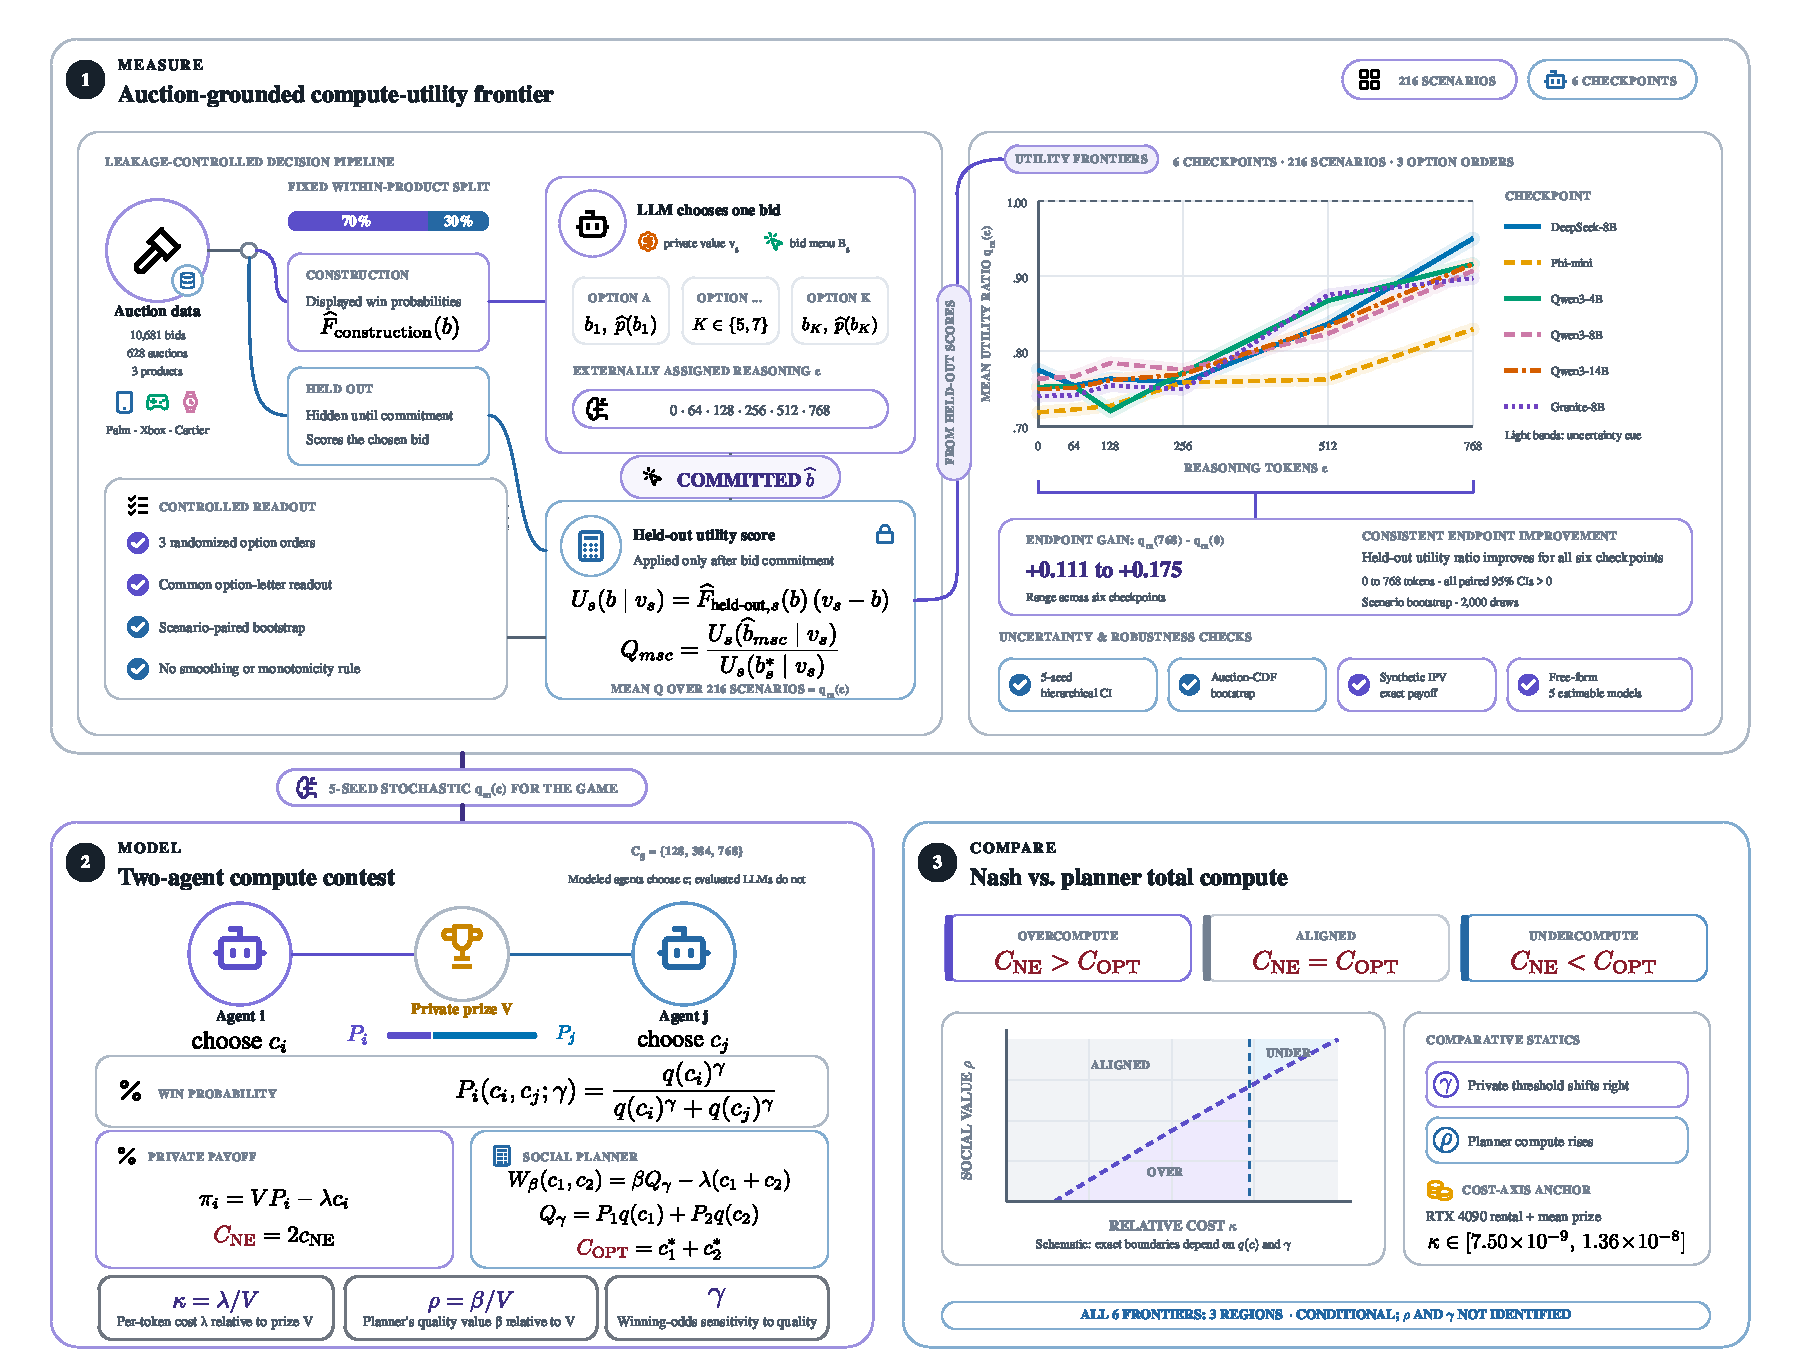
\includegraphics[width=0.94\linewidth]{figures/strategic_input_pipeline_overview.pdf}
\caption{Overview of the auction measurement and strategic-compute pipeline for the six-checkpoint analysis.}
\label{fig:pipelineoverview}
\end{figure}
\FloatBarrier

\section{Complete frontier and baseline results}
\label{app:fullresults}
Performance varies materially by product and option-set difficulty. At 768 tokens the category--width utility ratio ranges from 0.906 to 0.987 for DeepSeek-8B, 0.811 to 0.844 for Phi-mini, 0.860 to 0.967 for Qwen3-4B, 0.854 to 0.967 for Qwen3-8B, 0.829 to 0.982 for Qwen3-14B, and 0.868 to 0.917 for Granite-8B. Product, price scale, and auction support move together, so these are descriptive contrasts.
\paragraph{Calculator comparison and observable objective agreement.}
We audit all 23,328 greedy fixed-budget decisions, retaining the 216 scenarios and three option orders. Prompt-objective optimality uses the four-decimal probabilities actually displayed, reconstructed from the archived formatter. Held-out utility optimality permits payoff ties and therefore differs from exact-label accuracy. Each action belongs to one of four classes: optimal under both objectives, displayed-optimal only, held-out-optimal only, or suboptimal under both. These classes describe choices, not an internal arithmetic or reasoning mechanism.

The published full-precision construction calculator earns mean expected bidder profit of \$212.66 and mean held-out regret of \$3.09; it is utility-optimal on 155/216 scoring scenarios. Display precision changes its selected bid in one scenario, reducing mean profit by only \$0.0113. A separately recomputed calculator using exactly the displayed probabilities retains the same six-model simultaneous disadvantage for the LLMs. Thus the result does not depend on granting the calculator undisplayed precision.

For six 768-token model-minus-calculator profit gaps, 10,000 product-stratified value-family draws (seed 20261009) retain each family's four candidate variants and paired budget vectors, after averaging option orders. Exploratory simultaneous 95\% maximum-standardized-deviation bands all exclude zero. These draws condition on products, prompts and both CDFs; they do not add independent confirmation or stochastic-generation uncertainty to this greedy audit.

At 768 tokens, 42.1--86.3\% of choices maximize the displayed objective. Displayed-optimal but held-out-suboptimal choices comprise 9.4--22.8\%, while choices suboptimal under both comprise 11.9--52.0\%. The exact accounting identity is
\[
R_{\mathrm{model}}^{\mathrm{test}}=R_{\mathrm{calculator}}^{\mathrm{test}}+
\bigl(U_{\mathrm{calculator}}^{\mathrm{test}}-U_{\mathrm{model}}^{\mathrm{test}}\bigr).
\]
The second term is signed: model actions beat the calculator on held-out profit in 2.2--8.0\% of records, despite their aggregate disadvantage. Scoring-distribution differences can therefore reward a departure from the displayed objective. They do not explain all remaining action-selection losses. Supplementary product-level endpoints and regret concentration describe where gains and losses occur within these constructed tasks.
\begin{table}[htbp]
\centering\small
\caption{Calculator and observable-error audit of the greedy 768-token frontier. Profit differences are model minus construction-split calculator, with exploratory simultaneous 95\% family bands over six models. Displayed-optimal actions maximize profit under the four-decimal probabilities actually shown; held-out optimality admits payoff ties and differs from exact-label accuracy. All 216 scenarios and three option orders are retained.}
\label{tab:calculatorerroraudit}
\setlength{\tabcolsep}{4pt}
\begin{tabular}{lrrr}
\toprule
Model & Profit difference, USD [band] & Displayed-optimal (\%) & Both suboptimal (\%) \\
\midrule
DeepSeek-8B & -22.60 [-38.80, -6.39] & 86.3 & 11.9 \\
Phi-mini & -33.67 [-55.78, -11.57] & 42.1 & 52.0 \\
Qwen3-4B & -30.54 [-48.97, -12.11] & 71.1 & 25.6 \\
Qwen3-8B & -30.37 [-45.84, -14.91] & 67.7 & 28.1 \\
Qwen3-14B & -36.00 [-54.15, -17.86] & 76.7 & 20.5 \\
Granite-8B & -15.09 [-24.89, -5.28] & 53.5 & 41.2 \\
\bottomrule
\end{tabular}
\end{table}

% Automatically generated from replay/CPU CSV estimates. Requires booktabs and tabularx.
\begin{table}[htbp]
\caption{Exploratory paired 0-to-768 effects, conditional on three fixed products and the original prompts. 10,000 category-stratified category/value-family bootstrap draws; each family retains its four candidate variants. Intervals are pointwise.}
\label{tab:familyendpoints}
\centering
\small
\begin{tabularx}{\linewidth}{lXX}
\toprule
Model & Ratio gain [95\% family CI] & Profit gain, USD [95\% family CI] \\
\midrule
DeepSeek-8B & 0.175 [0.149, 0.202] & 29.61 [17.09, 45.28] \\
Phi-mini & 0.111 [0.085, 0.138] & 11.11 [4.36, 18.34] \\
Qwen3-4B & 0.164 [0.140, 0.189] & 30.47 [18.32, 44.22] \\
Qwen3-8B & 0.144 [0.119, 0.169] & 31.18 [17.00, 49.16] \\
Qwen3-14B & 0.167 [0.137, 0.197] & 31.57 [17.41, 48.75] \\
Granite-8B & 0.157 [0.123, 0.192] & 46.36 [25.46, 70.89] \\
\bottomrule
\end{tabularx}
\end{table}

\begin{table}[H]
\centering
\caption{Complete deterministic greedy frontier, averaged over 216 scenarios and three option orders. Accuracy is percent.}
\label{tab:fullgreedy}
\scriptsize
\setlength{\tabcolsep}{2.6pt}
\begin{tabular}{lrrrrrr}
\toprule
Model & 0 & 64 & 128 & 256 & 512 & 768 \\
\midrule
\multicolumn{7}{l}{\emph{Mean held-out utility ratio}}\\
DeepSeek-8B & .775 & .754 & .763 & .758 & .836 & .950 \\
Phi-mini & .718 & .722 & .727 & .758 & .762 & .829 \\
Qwen3-4B & .752 & .753 & .720 & .771 & .867 & .916 \\
Qwen3-8B & .763 & .766 & .784 & .775 & .823 & .907 \\
Qwen3-14B & .749 & .751 & .761 & .769 & .833 & .916 \\
Granite-8B & .740 & .741 & .754 & .749 & .875 & .897 \\
\midrule
\multicolumn{7}{l}{\emph{Exact-optimality rate (\%)}}\\
DeepSeek-8B & 21.5 & 20.4 & 21.9 & 21.0 & 38.7 & 64.7 \\
Phi-mini & 19.1 & 19.4 & 17.6 & 22.8 & 24.2 & 38.3 \\
Qwen3-4B & 21.1 & 22.8 & 20.4 & 22.1 & 42.3 & 57.4 \\
Qwen3-8B & 23.1 & 24.1 & 22.8 & 25.3 & 35.2 & 55.2 \\
Qwen3-14B & 23.8 & 24.4 & 24.1 & 30.7 & 42.1 & 59.6 \\
Granite-8B & 20.7 & 19.4 & 21.6 & 22.1 & 42.4 & 46.3 \\
\bottomrule
\end{tabular}
\end{table}

\begin{table}[H]
\centering
\caption{Analytic and generation controls, averaged over 216 scenarios. The unconstrained condition has a 1,024-token cap and is not budget-matched.}
\label{tab:baselines}
\small
\setlength{\tabcolsep}{4pt}
\begin{tabular}{lrrr}
\toprule
Policy or checkpoint & Utility ratio & Accuracy (\%) & Mean regret \\
\midrule
Held-out oracle & 1.000 & 100.0 & 0.000 \\
Construction-split calculator & 0.981 & 71.3 & 3.091 \\
Highest win probability & 0.731 & 28.2 & 81.319 \\
Median displayed position & 0.725 & 18.7 & 41.371 \\
Uniform random (expected) & 0.711 & 17.1 & 44.759 \\
\midrule
DeepSeek-8B unconstrained & 0.972 & 67.7 & 8.750 \\
Phi-mini unconstrained & 0.846 & 41.5 & 30.930 \\
Qwen3-4B unconstrained & 0.960 & 65.6 & 18.527 \\
Qwen3-8B unconstrained & 0.951 & 65.6 & 24.614 \\
Qwen3-14B unconstrained & 0.954 & 67.7 & 25.824 \\
Granite-8B unconstrained & 0.912 & 48.6 & 12.463 \\
\bottomrule
\end{tabular}
\end{table}

\begin{table}[H]
\centering
\caption{Five-seed stochastic frontier. Brackets give 95\% hierarchical-bootstrap intervals over scenarios and generation seeds.}
\label{tab:stochasticfrontier}
\scriptsize
\setlength{\tabcolsep}{3pt}
\begin{tabular}{lccc}
\toprule
Model & $q(128)$ & $q(384)$ & $q(768)$ \\
\midrule
DeepSeek-8B & .758 [.719,.791] & .777 [.738,.814] & .947 [.926,.966] \\
Phi-mini & .746 [.708,.785] & .744 [.708,.782] & .813 [.776,.848] \\
Qwen3-4B & .730 [.690,.768] & .803 [.771,.836] & .914 [.887,.938] \\
Qwen3-8B & .775 [.740,.808] & .795 [.757,.829] & .893 [.865,.917] \\
Qwen3-14B & .763 [.723,.799] & .793 [.754,.833] & .912 [.883,.941] \\
Granite-8B & .747 [.707,.783] & .805 [.766,.838] & .886 [.858,.913] \\
\bottomrule
\end{tabular}
\end{table}

\begin{table}[H]
\centering
\caption{Free-form readout sensitivity for the deterministic six-budget study. Validity is the share of parsed bids that match a displayed candidate; agreement is conditional on validity. Endpoint utility ratios use scenario--order cells valid at both 0 and 768 tokens. Intervals are 95\% scenario-bootstrap intervals for the paired difference.}
\label{tab:freeformsensitivity}
\scriptsize
\setlength{\tabcolsep}{3pt}
\begin{tabular}{lrrrrrr}
\toprule
Model & Valid (\%) & Agree (\%) & Paired scenarios & $q_{\mathrm{FF}}(0)$ & $q_{\mathrm{FF}}(768)$ & Difference (95\% CI) \\
\midrule
DeepSeek-8B & 66.8 & 46.6 & 197 & 0.739 & 0.969 & 0.230 [0.194, 0.270] \\
Phi-mini & 29.1 & 32.7 & 47 & 0.805 & 0.983 & 0.178 [0.117, 0.249] \\
Qwen3-4B & 74.3 & 54.5 & 169 & 0.740 & 0.954 & 0.215 [0.175, 0.254] \\
Qwen3-8B & 51.0 & 71.3 & 210 & 0.751 & 0.912 & 0.161 [0.133, 0.192] \\
\bottomrule
\end{tabular}
\end{table}

\begin{table}[H]
\centering
\caption{Available-case free-form diagnostics by assigned reasoning budget. Utility ratios average only valid parsed candidate bids at that budget and are therefore not compositionally balanced.}
\label{tab:freeformbybudget}
\scriptsize
\setlength{\tabcolsep}{3.8pt}
\begin{tabular}{llrrrrrr}
\toprule
Model & Statistic & 0 & 64 & 128 & 256 & 512 & 768 \\
\midrule
\multirow{2}{*}{DeepSeek-8B} & Validity (\%) & 99.2 & 73.8 & 56.5 & 42.6 & 66.0 & 62.5 \\
 & Utility ratio & .733 & .700 & .760 & .785 & .886 & .973 \\
\multirow{2}{*}{Phi-mini} & Validity (\%) & 62.8 & 42.4 & 21.5 & 17.7 & 15.9 & 14.2 \\
 & Utility ratio & .779 & .776 & .782 & .875 & .859 & .976 \\
\multirow{2}{*}{Qwen3-4B} & Validity (\%) & 99.5 & 96.6 & 67.7 & 69.3 & 53.2 & 59.3 \\
 & Utility ratio & .736 & .721 & .751 & .761 & .880 & .966 \\
\multirow{2}{*}{Qwen3-8B} & Validity (\%) & 98.3 & 2.8 & 6.5 & 42.1 & 68.1 & 88.0 \\
 & Utility ratio & .750 & .893 & .770 & .758 & .849 & .922 \\
\bottomrule
\end{tabular}
\end{table}


\FloatBarrier
\section{Strategic-game and compute-menu robustness}
\label{app:strategicrobustness}

The raw $(V,\lambda)$ grid and associated summaries in Tables~\ref{tab:strategicsensitivity}--\ref{tab:menurobustness} are reported as supplementary finite-grid diagnostics. Their bounds and weights were chosen before the monetary benchmark in Section~\ref{sec:monetarybenchmark}. We therefore reserve the substantive analysis for the normalized boundaries below.

Table~\ref{tab:normalizedthresholds} reports the exact $\gamma=1$ boundaries behind Figure~\ref{fig:normalizedphase}; the complete threshold CSV includes every tested $\gamma$. Under the specified contest, increasing $\gamma$ shifts the vertical private thresholds rightward and expands the overcompute region. Reporting boundaries avoids the dependence of phase-area percentages on pixel weights.

\begin{table}[H]
\centering
\caption{Exact compute-transition thresholds at $\gamma=1$ from the point stochastic frontiers. Nash entries are per-agent compute as $\kappa$ increases; planner entries are total compute as $r=\kappa/\rho=\lambda/\beta$ increases. Values are reduced-form game boundaries, not estimated market primitives.}
\label{tab:normalizedthresholds}
\scriptsize
\setlength{\tabcolsep}{3.0pt}
\begin{tabular}{llll}
\toprule
Model & Nash transition(s), $\kappa$ & Planner $1536\to896$, $\kappa/\rho$ & Planner $896\to256$, $\kappa/\rho$ \\
\midrule
DeepSeek-8B & $768\to128$: $8.65\times10^{-5}$ & $1.31\times10^{-4}$ & $1.64\times10^{-4}$ \\
Phi-mini & $768\to128$: $3.34\times10^{-5}$ & $4.99\times10^{-5}$ & $5.44\times10^{-5}$ \\
Qwen3-4B & $768\to384$: $8.39\times10^{-5}$; $384\to128$: $9.28\times10^{-5}$ & $1.27\times10^{-4}$ & $1.59\times10^{-4}$ \\
Qwen3-8B & $768\to128$: $5.49\times10^{-5}$ & $8.51\times10^{-5}$ & $9.80\times10^{-5}$ \\
Qwen3-14B & $768\to128$: $6.98\times10^{-5}$ & $1.07\times10^{-4}$ & $1.27\times10^{-4}$ \\
Granite-8B & $768\to384$: $6.27\times10^{-5}$; $384\to128$: $7.35\times10^{-5}$ & $1.00\times10^{-4}$ & $1.19\times10^{-4}$ \\
\bottomrule
\end{tabular}
\end{table}


\begin{figure}[t]
\centering
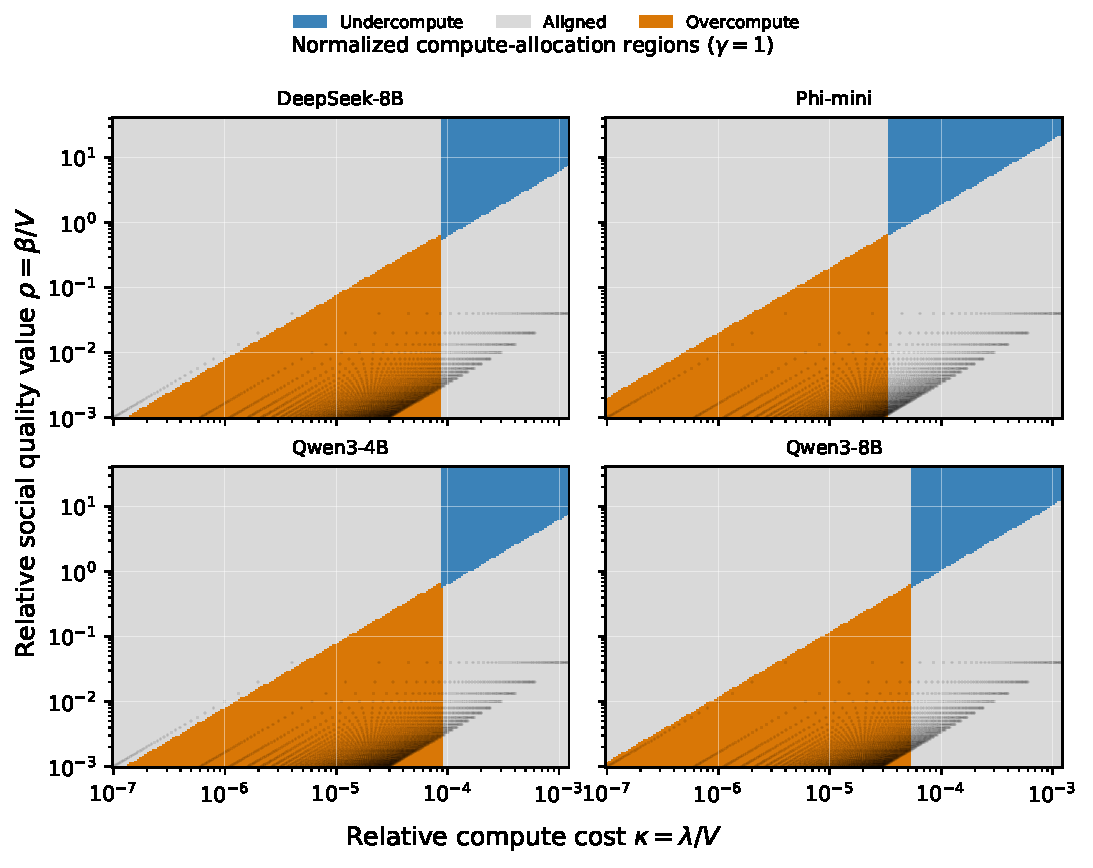
\includegraphics[width=0.76\linewidth]{figures/normalized_phase_gamma1.pdf}
\caption{Compute-allocation phase diagram implied by the stochastic three-budget frontier under the specified contest at $\gamma=1$. Colors compare total equilibrium and planner compute; faint points reproduce the raw $\beta=1$ grid.}
\label{fig:normalizedphase}
\end{figure}

\begin{figure}[t]
\centering
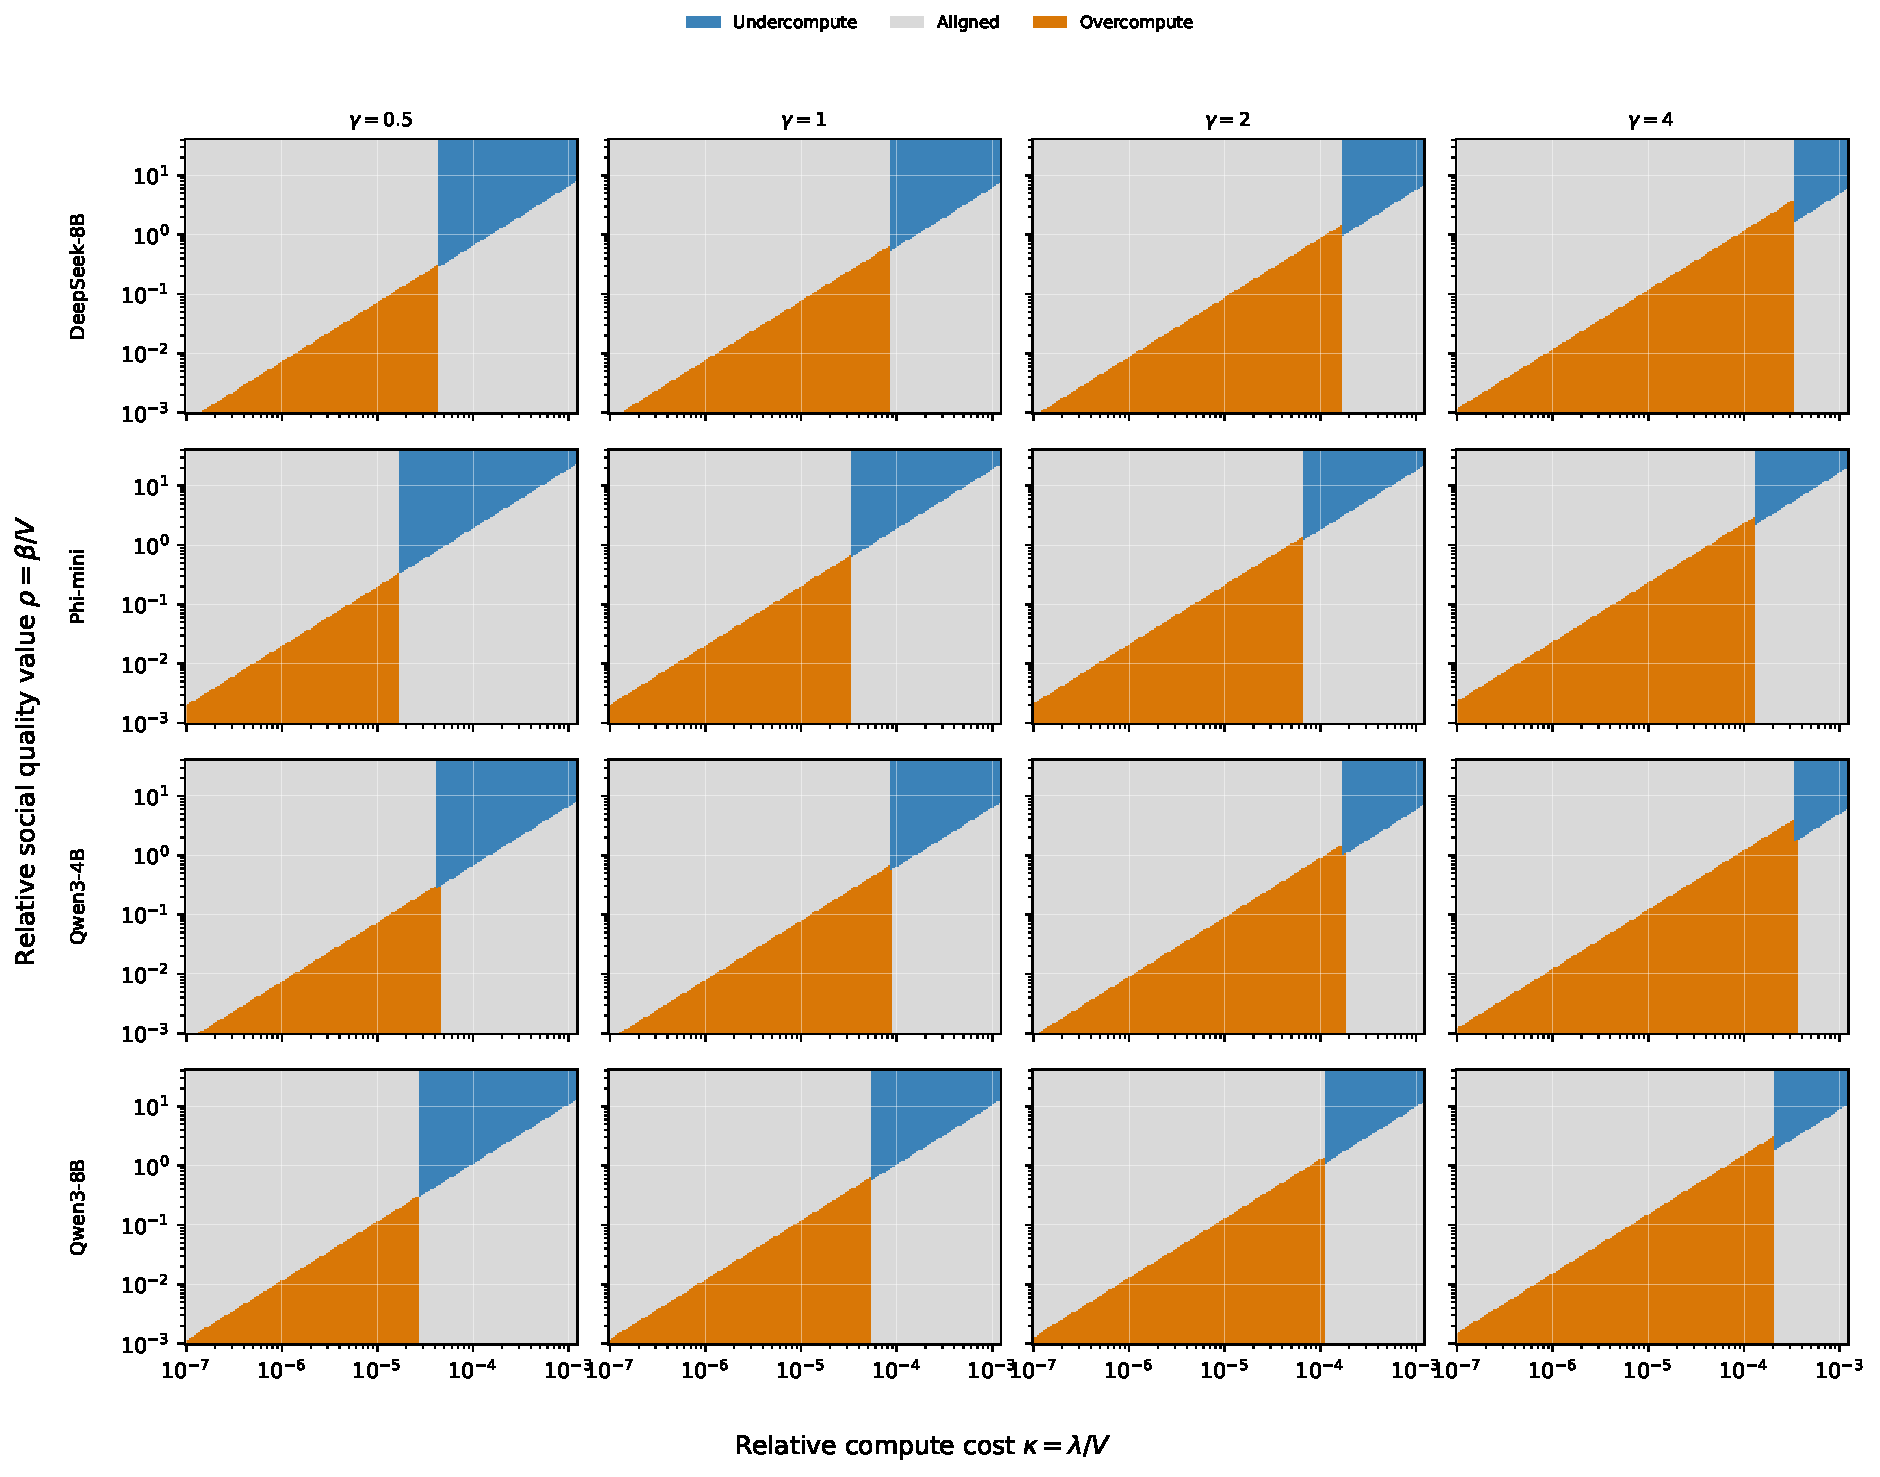
\includegraphics[width=0.98\linewidth]{figures/normalized_phase_all_gamma.pdf}
\caption{Normalized phase maps under the specified contest for every checkpoint and tested sensitivity $\gamma$. Axes and colors match Figure~\ref{fig:normalizedphase}. Each panel renders the symmetric-pure classification on a logarithmic grid; transition values are computed separately from payoff indifferences. The narrow Qwen3-4B mixed-only interval at $\gamma=4$ is resolved by the full equilibrium analysis in Appendix~\ref{app:completeequilibria}, not by the rendering grid.}
\label{fig:normalizedphasegamma}
\end{figure}

\subsection{Structural interpretation, full equilibria, and quality mapping}
\label{app:completeequilibria}

\paragraph{Why three regions can occur without a particular measured shape.}
Consider a finite menu with distinct budget costs, positive qualities, a strictly highest quality at the highest budget, and finite $\gamma>0$. At zero cost, the highest-quality action strictly dominates lower-quality actions under the Tullock rule. By finiteness and continuity, it remains dominant for sufficiently small positive $\kappa$. For sufficiently large $\kappa$, the cheapest action strictly dominates because selection gains are bounded. At fixed positive $\kappa$, the planner chooses the cheapest pair for sufficiently small $\rho$ and the highest/highest pair for sufficiently large $\rho$: every pair containing a lower-quality action has strictly lower expected selected quality. Low private cost with low social valuation therefore gives overcompute; high private cost with high valuation gives undercompute; the other extreme combinations give alignment. Strict choices persist on open neighborhoods. This argument requires a sufficiently broad parameter domain and the stated quality condition; a flat frontier instead gives cheapest-action alignment at every positive cost. It establishes model structure, not the prevalence of inefficient competition.

\paragraph{Complete equilibrium characterization.}
Index budgets by $a,b$, write $P_{ab}=q_a^\gamma/(q_a^\gamma+q_b^\gamma)$, and define $R_{ab}=P_{ab}-1/2-\kappa(c_a-c_b)$. Adding the rival's compute cost to each player's payoff leaves best responses unchanged and transforms the game into a constant-sum game. Since $P_{ab}+P_{ba}=1$, $R$ is skew symmetric and the zero-sum value is zero. Its common optimal-strategy polytope is
\begin{equation}
 \mathcal S(\kappa,\gamma)=\{x\geq0:\ \mathbf 1^\top x=1,\ Rx\leq0\}.
 \label{eq:equilibriumpolytope}
\end{equation}
The full Nash set is $\mathcal S\times\mathcal S$: any pair of strategies in this polytope is an equilibrium, including asymmetric pairs when the set is nontrivial. Vertices give the extrema of expected compute; vertex pairs give extrema of the bilinear expected modeled welfare. Consequently, selecting one symmetric mixture or one pure strategy at a tie need not describe all equilibrium compute or welfare outcomes.

The CPU analysis enumerates the polytope at payoff-indifference boundaries and on 160 open cost intervals across six point frontiers and four sensitivities, merging machine-precision duplicate cuts. Only one open interval lacks a pure equilibrium: Qwen3-4B at $\gamma=4$, between $\kappa=0.0003286027052518$ and $0.0003289091165272$. At the midpoint, the strategy over $\{128,384,768\}$ is $(0.00589117,0.00981862,0.98429020)$. An independent linear-programming solution agrees within $10^{-8}$; enumerated best-response residuals are below $10^{-9}$. Exact-boundary strategy multiplicity is retained in the machine-readable equilibrium regimes. This characterization applies to the symmetric service-prize contest, not automatically to asymmetric prizes or an endogenous auction game.

\paragraph{Quality scale and origin sensitivity.}
Multiplying every $q_a$ by a common positive constant preserves $P_{ab}$ and private incentives. It changes the planner quality units unless $\rho$ is rescaled reciprocally. Adding a constant instead changes contest advantages: Table~\ref{tab:qualityoriginsensitivity} holds costs, $\gamma$, and the menu fixed while adding 0.5 to each quality. The shifted score is a model diagnostic rather than a utility ratio or an estimated service-selection technology. Endpoint-matched illustrative shapes also move thresholds in the released mapping-sensitivity CSV. These comparisons make explicit which strategic predictions depend on frontier measurements and which depend on their economic interpretation.
\begin{table}[htbp]
\centering\small
\caption{Quality-origin sensitivity at $\gamma=1$. Entries are the relative-cost thresholds above which the maximum-budget symmetric equilibrium ceases. Costs and the menu are held fixed; the shift is illustrative, not estimated.}
\label{tab:qualityoriginsensitivity}
\begin{tabular}{lrrr}
\toprule
Model & Measured $q$ & Shifted $q+0.5$ & Reduction (\%) \\
\midrule
DeepSeek-8B & $8.655\times10^{-5}$ & $5.455\times10^{-5}$ & 37.0 \\
Phi-mini & $3.344\times10^{-5}$ & $2.037\times10^{-5}$ & 39.1 \\
Qwen3-4B & $8.393\times10^{-5}$ & $5.304\times10^{-5}$ & 36.8 \\
Qwen3-8B & $5.489\times10^{-5}$ & $3.432\times10^{-5}$ & 37.5 \\
Qwen3-14B & $6.984\times10^{-5}$ & $4.373\times10^{-5}$ & 37.4 \\
Granite-8B & $6.273\times10^{-5}$ & $3.942\times10^{-5}$ & 37.2 \\
\bottomrule
\end{tabular}
\end{table}


\paragraph{Economic scoring versus accuracy and illustrative shape.}
Table~\ref{tab:metricshapecomparison} separates two substitutions on the same stochastic three-budget menu. First, the accuracy frontier replaces utility ratio in contract selection while keeping $\gamma=1$ and private cost $\kappa$ fixed. Second, an endpoint-matched linear utility frontier retains $q(128)$ and $q(768)$ and sets $q(384)=q(128)+0.4[q(768)-q(128)]$. For any positive score, 768/768 remains a pure equilibrium up to
\[
\min_{a\in\{128,384\}}
\frac{\tfrac12-q(a)/(q(a)+q(768))}{768-a},
\]
obtained by checking both lower-budget deviations against a 768-token rival. Point comparisons use saved frontiers; the paired uncertainty extension below uses the same preserved decisions without new inference.

The accuracy substitution changes the absolute score level and relative gains; it does not isolate frontier shape. At point estimates, the linear substitution preserves the measured endpoints and has modest effects on this boundary. Together with the flat-frontier counterexample above, these comparisons distinguish conditional numerical content from generic three-region existence.

In the DeepSeek-8B example, 128 strictly dominates both other budgets under utility-based selection at $\kappa=1.5\times10^{-4}$, whereas 768 strictly dominates under accuracy-based selection. Thus each reported equilibrium is unique, including mixed strategies. This hypothetical cost is outside the illustrative monetary anchor. The example demonstrates that changing the selection score can change compute prescriptions within the model, not that one score is an empirically correct service technology. No planner comparison is inferred: replacing quality by accuracy would also change client-value units, requiring a separate justification or adjustment of $\rho$.
\begin{table}[htbp]
\centering\small
\caption{Metric and shape sensitivity with paired uncertainty at $\gamma=1$. The threshold supports the 768/768 pure equilibrium. Accuracy/utility and linear change are point estimates. The accuracy-minus-utility threshold difference has exploratory simultaneous 95\% bands over six models, in units of $10^{-4}$; all bands exclude zero. The bootstrap uses 10,000 product-stratified family/seed draws, retaining all draws.}
\label{tab:metricshapecomparison}
\setlength{\tabcolsep}{4pt}
\begin{tabular}{lrrrr}
\toprule
Model & Utility threshold & Accuracy/utility & Difference [simult. band] & Linear change (\%) \\
\midrule
DeepSeek-8B & $8.65\times10^{-5}$ & 5.04 & 3.49 [2.39, 4.59] & -4.24 \\
Phi-mini & $3.34\times10^{-5}$ & 5.96 & 1.66 [0.26, 3.06] & -1.68 \\
Qwen3-4B & $8.39\times10^{-5}$ & 4.63 & 3.05 [1.92, 4.18] & -0.52 \\
Qwen3-8B & $5.49\times10^{-5}$ & 5.89 & 2.69 [1.50, 3.87] & -2.73 \\
Qwen3-14B & $6.98\times10^{-5}$ & 4.45 & 2.41 [1.51, 3.31] & -3.45 \\
Granite-8B & $6.27\times10^{-5}$ & 4.05 & 1.91 [0.64, 3.18] & +3.12 \\
\bottomrule
\end{tabular}
\end{table}


\paragraph{Paired uncertainty and allocation stability.}
We use 10,000 draws (seed 20261008). Within each fixed product, 18 product/private-value families are sampled with replacement, retaining all four candidate variants. Each selected scenario occurrence samples one of its five generation seeds, jointly across budgets and metrics, independently across models. Family selections are shared across models. This preserves paired decisions and family dependence while incorporating stored generation variation. The six accuracy-minus-utility threshold differences receive exploratory simultaneous 95\% maximum-standardized-deviation bands. All lower bounds are positive. Products, original prompts and scoring CDFs remain fixed; these bands exclude market shift, construction-split uncertainty and model misspecification.

The DeepSeek strict-dominance contrast persists in all 10,000 draws, a bootstrap stability frequency rather than a posterior or market probability. Twelve Phi utility draws have nonpositive high/high indifference bounds, meaning 768/768 lacks support at positive cost; absolute-difference bands retain those draws. Supplementary ratio intervals condition on positive utility bounds and are labelled separately. Linear-minus-measured threshold intervals exclude zero only for DeepSeek and Qwen3-14B. Four include zero, and Qwen3-4B and Granite exhibit substantial upper-tail shape sensitivity. Small point changes therefore do not establish that intermediate shape is generally unimportant.

\paragraph{Alternative client value and selection rules.}
A profit-based alternative uses $q_m^{\$}(c)=\overline U_m(c)/\overline U^*$, where $\overline U^*$ is mean oracle profit on the same constructed scenarios. This weights dollar consequences rather than normalizing each scenario separately. If a client values the selected recommendation by its predicted bidder profit, service benefit is $\overline U_m(c)=\overline U^*q_m^{\$}(c)$. Summing client profit net of the contract payment with provider profit gives selected expected bidder profit minus both compute costs. This specification provides explicit client-value units, conditional on benchmark profit predicting service benefit; it remains distinct from auction total surplus, which includes the seller. It neither identifies service payment nor demonstrates external validity.

A second alternative models noisy client comparison of quality differences. Assume a logistic noise term with fixed scale $s_m=\overline q_m$, the mean of the three point utility scores. Then selection probability is
\[
P_i^{L}(c_i,c_j)=\{1+\exp[-(q_m(c_i)-q_m(c_j))/s_m]\}^{-1}.
\]
At equal reference qualities, its slope in the quality difference is $1/(4\overline q_m)$, matching the Tullock $\gamma=1$ slope. With $s_m$ held fixed, a common origin shift leaves selection unchanged. This is a sensitivity specification, not a fitted client-choice model; the reference scale is frozen across draws to isolate frontier uncertainty.

Table~\ref{tab:selectionmappings} reports private high/high bounds. Profit-based point thresholds are 0.24--1.85 times the utility thresholds, and high/high support disappears in 24.71\% of Phi, 36.68\% of Qwen3-4B, 9.42\% of Qwen3-8B and 0.06\% of Granite draws. Matched logit point thresholds increase by 1.40--4.28\%. Halving or doubling discrimination instead gives about 0.51--0.52 or 2.01--2.07 times the original thresholds. Thus both the score's economic weighting and the client's discrimination assumption matter. No common-$\rho$ planner comparison is inferred across different client-value units.
\begin{table}[htbp]
\centering\small
\caption{Alternative selection assumptions on the same stochastic menu. Profit quality is mean expected bidder profit divided by mean oracle profit. Its signed high/high indifference bound has pointwise 95\% family/seed intervals, in units of $10^{-4}$; a nonpositive bound gives no high/high equilibrium at positive cost. Unsupported-draw percentages retain every draw. The matched logit uses fixed noise scale $s=\overline q_m$, matching the Tullock $\gamma=1$ local slope at equal reference quality. Ratios are point estimates; these alternatives are not fitted client behavior.}
\label{tab:selectionmappings}
\setlength{\tabcolsep}{3.5pt}
\begin{tabular}{lrrrr}
\toprule
Model & Profit/utility & Profit bound [95\% CI] & Unsupported (\%) & Logit/utility \\
\midrule
DeepSeek-8B & 1.09 & 0.94 [0.58, 1.39] & 0.00 & 1.03 \\
Phi-mini & 0.59 & 0.20 [-0.34, 0.55] & 24.71 & 1.01 \\
Qwen3-4B & 0.24 & 0.20 [-0.56, 0.66] & 36.68 & 1.04 \\
Qwen3-8B & 0.52 & 0.29 [-0.15, 0.72] & 9.42 & 1.01 \\
Qwen3-14B & 1.00 & 0.70 [0.34, 1.08] & 0.00 & 1.02 \\
Granite-8B & 1.85 & 1.16 [0.40, 1.84] & 0.06 & 1.04 \\
\bottomrule
\end{tabular}
\end{table}


\subsection{Zero-compute-augmented game sensitivity}
\label{app:zeroaugmented}

The primary game intentionally retains the clean five-seed stochastic menu $\mathcal C_S=\{128,384,768\}$. The zero-action sensitivity instead uses the hybrid menu $\mathcal C_H=\{0,128,384,768\}$. For each model and scenario, $Q^H_{m,s,0}$ is the mean of the stored deterministic reasoning-mode $c=0$ measurements over option-order seeds $\{11,23,37\}$. At positive budgets we retain, without smoothing, the stored stochastic measurements from seeds $\{1,7,21,42,99\}$ at fixed option-order seed 314159. Granite-8B's point hybrid frontier is $(0.7404,0.7466,0.8050,0.8865)$; the complete six-model panel is released as CSV.

This construction combines two protocols. The zero action comes from deterministic order replications, while positive actions come from stochastic decoding under one fixed presentation order. The result is an approximate sensitivity check on the availability of zero compute; a clean four-budget stochastic frontier would require a matched protocol.

We enumerate $\mathcal C_H\times\mathcal C_H$ exactly under the same normalized payoff, contest rule, and tie-breaking conventions for every $\gamma\in\{0.5,1,2,4\}$. Table~\ref{tab:zeroaugmented} gives the $\gamma=1$ transitions and Figure~\ref{fig:zeroaugmented} compares its phase map directly with the primary game. For Granite-8B, Nash compute moves $768\to0$ at $\kappa=5.83\times10^{-5}$, while planner total compute moves $1536\to768\to0$ at $r=8.69\times10^{-5}$ and $1.04\times10^{-4}$. Despite these shifts, the specified contest retains overcompute, aligned, and undercompute open regions for all six point frontiers at every tested $\gamma$.

\begin{table}[H]
\centering
\caption{Exact $\gamma=1$ transition comparison. Nash entries are per-agent compute as $\kappa$ increases; hybrid planner entries are total compute as $r=\kappa/\rho$ increases. ``Preserved'' means that overcompute, aligned, and undercompute open regions all remain; it is not a statement about phase-map area.}
\label{tab:zeroaugmented}
\scriptsize
\setlength{\tabcolsep}{3pt}
\begin{tabular}{@{}lp{0.20\linewidth}p{0.22\linewidth}p{0.31\linewidth}c@{}}
\toprule
Model & Primary Nash & Zero-augmented Nash & Zero-augmented planner & Three regions? \\
\midrule
DeepSeek-8B & $768\to128$: $8.65\!\times\!10^{-5}$ & $768\to0$: $6.48\!\times\!10^{-5}$ & $1536\to768$: $1.00\!\times\!10^{-4}$; $768\to0$: $1.23\!\times\!10^{-4}$ & Preserved \\
Phi-mini & $768\to128$: $3.34\!\times\!10^{-5}$ & $768\to128$: $3.34\!\times\!10^{-5}$; $128\to0$: $7.44\!\times\!10^{-5}$ & $1536\to896$: $4.99\!\times\!10^{-5}$; $896\to256$: $5.44\!\times\!10^{-5}$; $256\to128$: $1.07\!\times\!10^{-4}$; $128\to0$: $1.11\!\times\!10^{-4}$ & Preserved \\
Qwen3-4B & $768\to384$: $8.39\!\times\!10^{-5}$; $384\to128$: $9.28\!\times\!10^{-5}$ & $768\to0$: $6.33\!\times\!10^{-5}$ & $1536\to768$: $9.52\!\times\!10^{-5}$; $768\to0$: $1.16\!\times\!10^{-4}$ & Preserved \\
Qwen3-8B & $768\to128$: $5.49\!\times\!10^{-5}$ & $768\to0$: $5.10\!\times\!10^{-5}$ & $1536\to768$: $7.79\!\times\!10^{-5}$; $768\to0$: $9.11\!\times\!10^{-5}$ & Preserved \\
\bottomrule
\end{tabular}%
\end{table}


\begin{figure}[H]
\centering
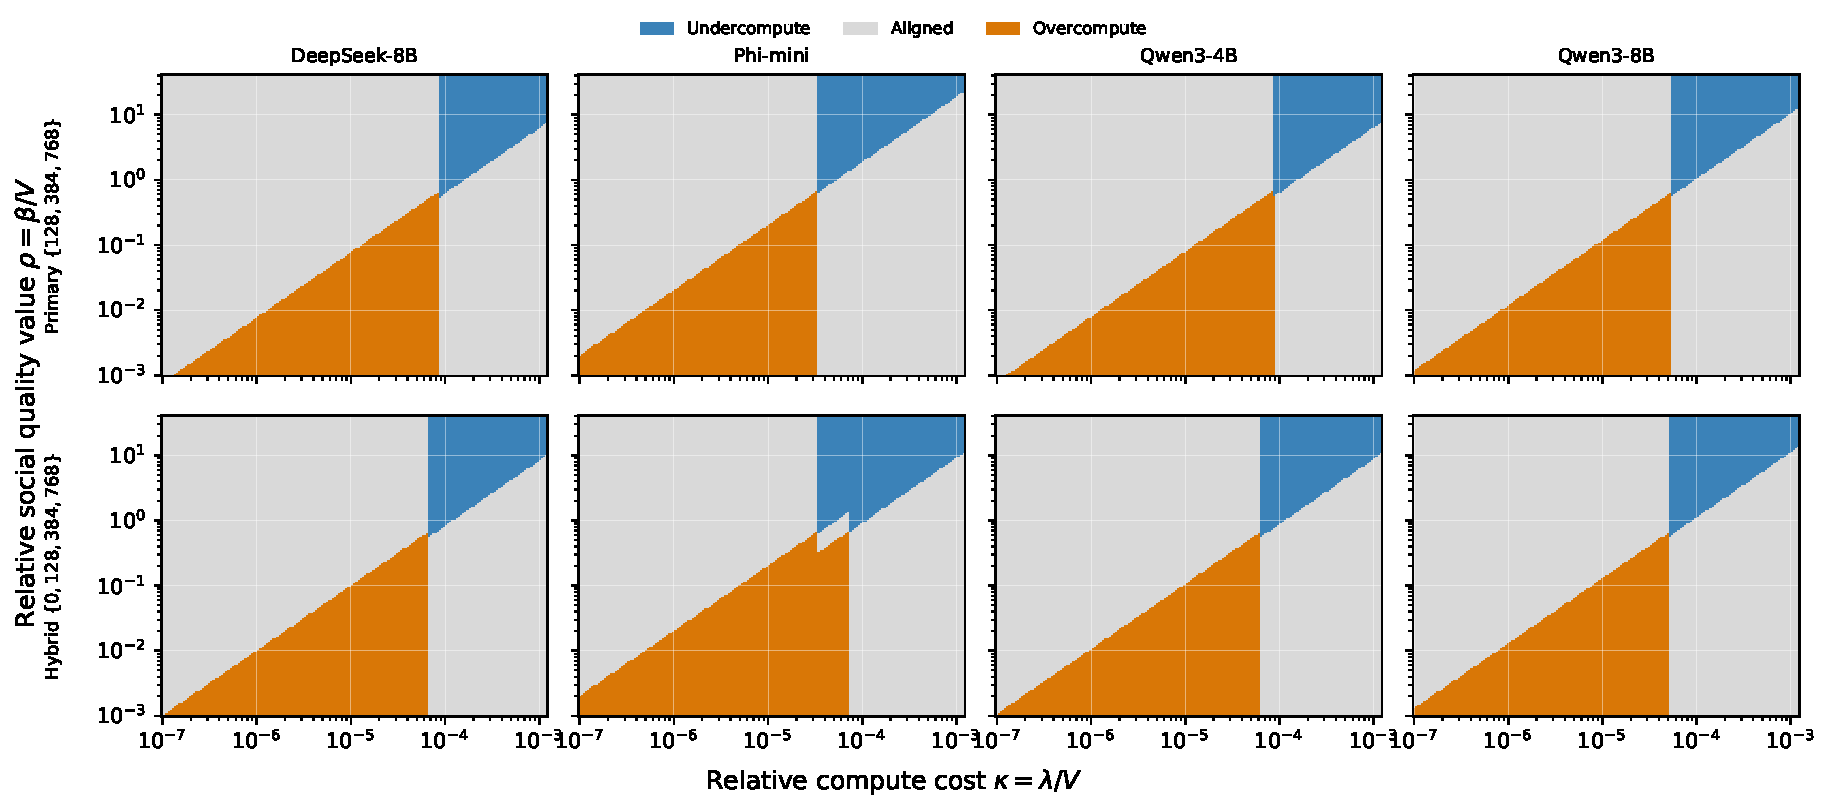
\includegraphics[width=0.98\linewidth]{figures/hybrid_zero_compute_phase_comparison_gamma1.pdf}
\caption{Direct comparison of allocations implied by the primary stochastic frontier and zero-compute-augmented sensitivity under the specified contest at $\gamma=1$. Axes and colors match Figure~\ref{fig:normalizedphase}. Pixel area serves only as a rendering device; conclusions use exact transition boundaries.}
\label{fig:zeroaugmented}
\end{figure}

The hybrid bootstrap resamples scenarios jointly across all four actions. A selected scenario contributes its deterministic order-averaged zero value; one of its five stored stochastic seeds is then sampled and used jointly at 128, 384, and 768 tokens. We recompute the exact game in each of 1,000 draws. All three phase types occur as open regions for all six models and all four $\gamma$ values in every draw. A subset of resampled frontiers produces a narrow interval without a symmetric pure equilibrium under the paper's selection rule (0--11.3\% of draws across model--$\gamma$ combinations), and we flag those intervals separately. The machine-readable output gives each boundary's presence frequency and a conditional interval when it appears. Joint resampling preserves the available scenario dependence, while the underlying protocol mismatch remains.

Figure~\ref{fig:strategicsensitivity} plots one-parameter slices of the retained raw grid. At fixed $(V,\lambda)$, $\beta$ enters through $\rho$, so equilibrium compute stays fixed while planner compute rises. At high $\rho$, positive welfare loss can coexist with zero excess-compute share because equilibrium compute is below the planner allocation. The fixed $0.01$ exclusion used in the supplementary relative-loss table is scale dependent and plays no role in the normalized phase analysis.

\begin{figure}[H]
\centering
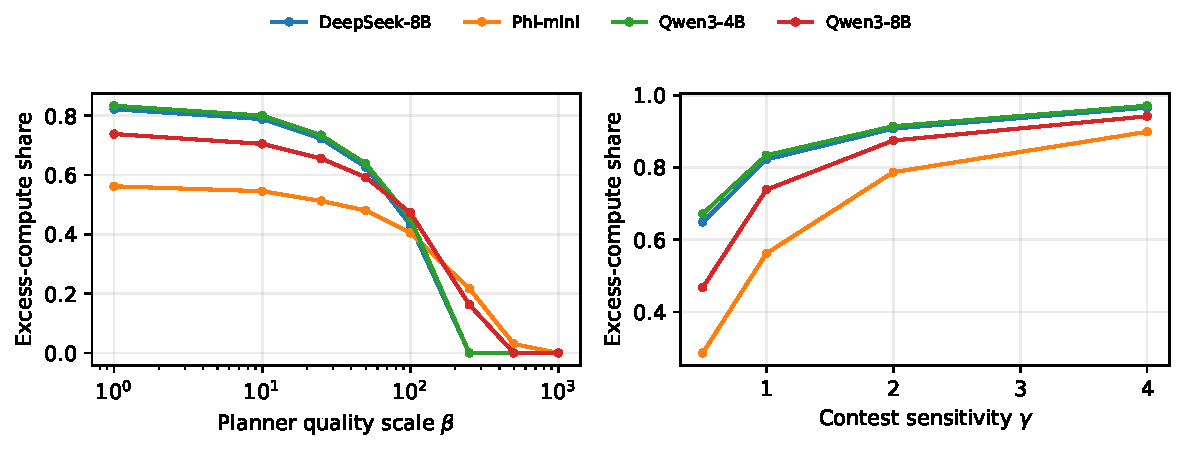
\includegraphics[width=0.88\linewidth]{figures/strategic_parameter_sensitivity.pdf}
\caption{Point-estimate strategic sensitivity on the primary stochastic frontier. The left panel varies planner quality scale with $\gamma=1$; the right varies contest sensitivity with $\beta=1$.}
\label{fig:strategicsensitivity}
\end{figure}

\begin{table}[H]
\centering
\caption{Legacy-scale comparative statics using the point stochastic frontier. Entries are ranges across checkpoints on the previously declared 2,400-cell $(V,\lambda)$ grid. At fixed $(V,\lambda)$, changing $\beta$ changes $\rho=\beta/V$ while holding $\kappa=\lambda/V$ fixed. Aggregate shares and means remain grid dependent; $\Delta W$ is in original $W_\beta$ units.}
\label{tab:strategicsensitivity}
\small
\setlength{\tabcolsep}{3.2pt}
\begin{tabular}{lrrrr}
\toprule
Setting & Excess share (\%) & $\Delta W$ & $C_{\mathrm{NE}}$ & $C_{\mathrm{OPT}}$ \\
\midrule
$\beta=1$ & 56.2--83.4 & 7.84--14.90 & 975.5--1331.1 & 256.0--277.3 \\
$\beta=10$ & 54.5--80.0 & 7.51--13.57 & 975.5--1331.1 & 277.3--330.7 \\
$\beta=25$ & 51.2--73.5 & 6.99--11.50 & 975.5--1331.1 & 320.0--416.0 \\
$\beta=50$ & 48.0--64.4 & 6.16--8.84 & 975.5--1331.1 & 373.3--565.3 \\
$\beta=100$ & 40.5--49.1 & 3.92--5.61 & 975.5--1331.1 & 480.0--885.3 \\
$\beta=250$ & 0.0--21.8 & 2.03--3.37 & 975.5--1331.1 & 810.7--1536.0 \\
$\beta=500$ & 0.0--3.0 & 3.62--10.99 & 975.5--1331.1 & 1365.3--1536.0 \\
$\beta=1000$ & 0.0--0.0 & 17.84--26.21 & 975.5--1331.1 & 1536.0--1536.0 \\
\midrule
$\gamma=0.5$ & 28.7--67.2 & 2.02--10.49 & 623.5--1111.0 & 256.0--277.3 \\
$\gamma=1$ & 56.2--83.4 & 7.84--14.90 & 975.5--1331.1 & 256.0--277.3 \\
$\gamma=2$ & 78.7--91.4 & 13.64--17.10 & 1263.5--1441.1 & 256.0--277.3 \\
$\gamma=4$ & 89.9--97.1 & 16.52--18.20 & 1406.4--1495.1 & 256.0--266.7 \\
\bottomrule
\end{tabular}
\end{table}

\begin{table}[H]
\centering
\caption{Secondary summary on the previously declared raw $(V,\lambda)$ grid, using the stochastic frontier on $\{128,384,768\}$ with $\beta=\gamma=1$. Intervals are 95\% hierarchical-bootstrap intervals over scenarios and generation seeds; PoRC is conditional on excess compute and is menu dependent.}
\label{tab:game}
\small
\setlength{\tabcolsep}{4pt}
\begin{tabular}{lcc}
\toprule
Model & Excess-compute share (95\% CI) & PoRC diagnostic (95\% CI) \\
\midrule
DeepSeek-8B & 82.21\% [78.33, 85.21] & 6.000 [6.000, 6.000] \\
Phi-mini & 56.21\% [18.29, 74.88] & 6.000 [5.571, 6.000] \\
Qwen3-4B & 83.38\% [77.88, 90.08] & 5.937 [5.412, 6.000] \\
Qwen3-8B & 73.83\% [63.04, 79.13] & 6.000 [5.898, 6.000] \\
Qwen3-14B & 78.04\% [73.42, 82.46] & 6.000 [5.905, 6.000] \\
Granite-8B & 80.75\% [70.83, 87.71] & 5.782 [4.906, 6.000] \\
\bottomrule
\end{tabular}
\end{table}

\begin{table}[H]
\centering
\caption{Legacy welfare-loss summary on the previously declared raw $(V,\lambda)$ grid at $\beta=\gamma=1$. Absolute values are in the original $W_\beta$ units, not market-identified dollars or scale-invariant normalized loss. Intervals are 95\% hierarchical-bootstrap intervals; relative loss uses the legacy, non-scale-invariant omission rule $|W_{\mathrm{OPT}}|\leq0.01$.}
\label{tab:welfareuncertainty}
\small
\setlength{\tabcolsep}{3.5pt}
\begin{tabular}{lcc}
\toprule
Model & Mean absolute loss (95\% CI) & Mean relative loss (95\% CI) \\
\midrule
DeepSeek-8B & 14.868 [13.898, 15.608] & 7.642 [7.389, 10.153] \\
Phi-mini & 7.842 [0.807, 12.364] & 5.752 [3.159, 7.128] \\
Qwen3-4B & 14.902 [13.470, 15.650] & 7.344 [7.081, 8.941] \\
Qwen3-8B & 12.343 [9.597, 13.963] & 7.859 [5.329, 10.814] \\
\bottomrule
\end{tabular}
\end{table}

\begin{table}[H]
\centering
\caption{Compute-menu/frontier sensitivity. The three-budget rows use the primary five-seed stochastic frontier; the six-budget rows use the order-averaged deterministic frontier and therefore change both menu and decoding regime. Six-budget intervals are 95\% scenario-bootstrap intervals.}
\label{tab:menurobustness}
\small
\setlength{\tabcolsep}{3.0pt}
\begin{tabular}{llrrr}
\toprule
Model & Menu/frontier & Excess share (95\% CI) & $C_{\mathrm{NE}}$ & $C_{\mathrm{OPT}}$ \\
\midrule
DeepSeek-8B & Stoch. 3 & 82.2 [78.3, 85.2] & 1329.6 & 277.3 \\
             & Determ. 6 & 76.8 [74.1, 80.1] & 1205.1 & 25.6 \\
Phi-mini    & Stoch. 3 & 56.2 [18.3, 74.9] & 975.5 & 256.0 \\
             & Determ. 6 & 72.3 [58.6, 93.5] & 1056.9 & 0.0 \\
Qwen3-4B    & Stoch. 3 & 83.4 [77.9, 90.1] & 1331.1 & 277.3 \\
             & Determ. 6 & 79.5 [73.6, 84.3] & 1189.5 & 12.8 \\
Qwen3-8B    & Stoch. 3 & 73.8 [63.0, 79.1] & 1201.1 & 256.0 \\
             & Determ. 6 & 74.4 [68.3, 92.6] & 1143.0 & 12.8 \\
\bottomrule
\end{tabular}
\end{table}


\FloatBarrier
\section{Held-out auction-CDF uncertainty}
\label{app:auctioncdf}

Within each product, an auction bootstrap samples the held-out closing prices with replacement, recomputes the empirical probability of clearing every stored candidate bid, and re-scores the fixed constrained choices and the best candidate. The three option-order choices are averaged within scenario--budget cells before aggregation. This procedure holds the 216 tasks fixed and varies the finite held-out CDF, making it orthogonal to both scenario and generation resampling. Responses to probabilities from a new construction split remain beyond its scope.

\begin{table}[H]
\centering
\caption{Held-out auction-CDF uncertainty. Each of 2,000 draws resamples held-out auctions within product and re-scores the fixed stored deterministic choices. Intervals therefore capture closing-price-CDF estimation only, not scenario composition, decoding, or responses to alternative displayed construction CDFs.}
\label{tab:auctioncdf}
\small
\setlength{\tabcolsep}{4pt}
\begin{tabular}{lrrr}
\toprule
Model & $q(0)$ & $q(768)$ & Difference (95\% CI) \\
\midrule
DeepSeek-8B & 0.767 & 0.937 & 0.171 [0.152, 0.187] \\
Phi-mini & 0.708 & 0.818 & 0.111 [0.092, 0.130] \\
Qwen3-4B & 0.744 & 0.904 & 0.160 [0.146, 0.173] \\
Qwen3-8B & 0.755 & 0.895 & 0.140 [0.128, 0.150] \\
Qwen3-14B & 0.742 & 0.904 & 0.161 [0.143, 0.175] \\
Granite-8B & 0.733 & 0.885 & 0.152 [0.132, 0.168] \\
\bottomrule
\end{tabular}
\end{table}


\FloatBarrier
\section{Synthetic IPV robustness}
\label{app:syntheticipv}

The historical benchmark estimates winning probabilities from auction records. As a separate check, we evaluate the same six checkpoints in a synthetic independent-private-values first-price auction with exact payoffs. Each focal bidder faces two opponents whose values are independent discrete uniforms on $\{0,\ldots,99\}$ and whose bids follow $b(v)=2v/3$. Win probabilities enumerate all 10,000 opponent-value pairs and split highest-bid ties uniformly. The 216 scenarios cross five- and seven-option menus with structured and unstructured candidate sets; private values span 8--99. Candidate sets are generated before utilities are evaluated and therefore do not condition on the optimal bid.

The deterministic study uses budgets $\{0,64,128,256,384,512,768\}$ and option-order seeds $\{11,23,37\}$. Every model contributes 4,536 valid records, with no missing cells, duplicate keys, invalid constrained choices, non-finite scores, or token-count violations. All six files share benchmark hash \nolinkurl{f252c795796370bcbe6e291df8737011a87d7f68f0e3a367de475c53fecff4fb}. Granite retains the protocol difference described in Section~4.2.

\begin{table}[H]
\centering
\caption{Wall-clock and monetary cost of the synthetic IPV sweep.}
\label{tab:syntheticruntimecost}
\small
\setlength{\tabcolsep}{4pt}
\begin{tabular}{@{}lccccc@{}}
\toprule
Model & GPU & Full run & Mean/cell & Mean at 768 & Cost (\$) \\
\midrule
Phi-mini       & RTX 4090 & 4:37:23  & 3.66 s  & 9.15 s  & 3.42 \\
Qwen3-4B       & RTX 4090 & 5:37:54  & 4.46 s  & 10.87 s & 4.17 \\
DeepSeek-8B    & RTX 4090 & 7:55:22  & 6.28 s  & 15.44 s & 5.86 \\
Qwen3-8B       & RTX 4090 & 8:39:31  & 6.86 s  & 16.75 s & 6.41 \\
Granite-8B     & RTX 4090 & 8:56:45  & 7.09 s  & 17.19 s & 6.62 \\
Qwen3-14B      & L40S     & 17:57:14 & 14.23 s & 34.80 s & 17.95 \\
\midrule
Sequential total & -- & 53:44:09 & -- & -- & 44.43 \\
\bottomrule
\end{tabular}
\end{table}

These are end-to-end wall-clock measurements within each timed sweep and each recorded cell: they include prompt processing, reasoning generation, the free-form answer stage, and constrained readout. Model loading preceded the sweep timer and is excluded. Costs multiply the exact unrounded run durations by RunPod on-demand accounting rates of \$0.74 per GPU-hour for the RTX~4090 and \$1.00 for the L40S \citep{runpod2026pricing}, with only the displayed totals rounded to cents. These totals differ from $\lambda$ in Section~\ref{sec:monetarybenchmark}: $\lambda$ is the incremental cost per additional reasoning token, estimated from a runtime regression and used to calibrate the contest, whereas Table~\ref{tab:syntheticruntimecost} prices the complete sweep. Accordingly, the 768-token cell means include a fixed intercept and prompt, answer, and readout overhead; they also summarize deterministic synthetic runs rather than the stochastic auction records used for the marginal slopes. Qwen3-14B ran on an L40S while the other five models ran on RTX~4090 GPUs, so its elapsed time and cost are not a hardware-controlled comparison with the rest of the panel.

\begin{table}[H]
\centering
\caption{Synthetic IPV endpoint robustness over 216 paired scenarios. Intervals are 95\% paired scenario-bootstrap intervals for $q(768)-q(0)$ based on 2,000 draws.}
\label{tab:syntheticipv}
\small
\setlength{\tabcolsep}{4pt}
\begin{tabular}{lrrr}
\toprule
Model & $q(0)$ & $q(768)$ & Difference (95\% CI) \\
\midrule
DeepSeek-8B & 0.699 & 0.981 & 0.282 [0.247, 0.321] \\
Phi-mini & 0.651 & 0.815 & 0.164 [0.132, 0.197] \\
Qwen3-4B & 0.686 & 0.971 & 0.285 [0.248, 0.325] \\
Qwen3-8B & 0.704 & 0.956 & 0.253 [0.215, 0.293] \\
Qwen3-14B & 0.705 & 0.993 & 0.288 [0.246, 0.331] \\
Granite-8B & 0.664 & 0.881 & 0.217 [0.176, 0.259] \\
\bottomrule
\end{tabular}
\end{table}


\begin{figure}[H]
\centering
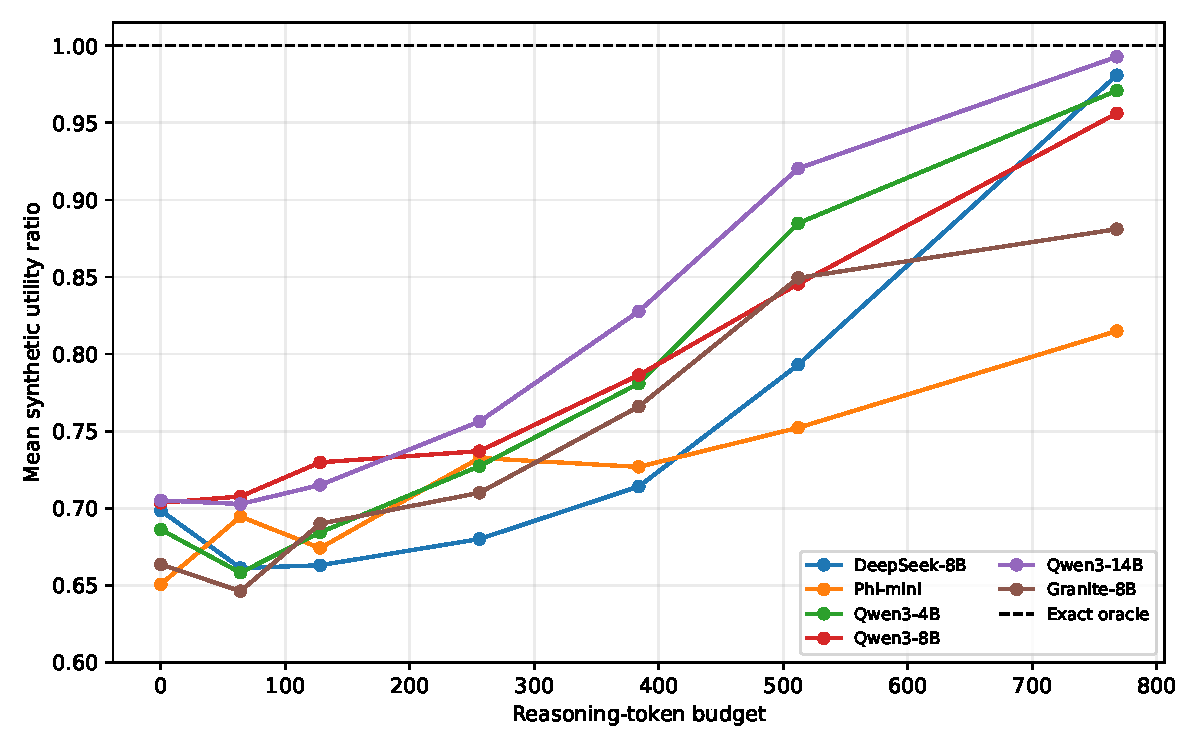
\includegraphics[width=0.88\linewidth]{figures/synthetic_ipv_six_model_frontier.pdf}
\caption{Six-model deterministic frontiers on the synthetic IPV benchmark. Lines join evaluated budgets without smoothing or a monotonicity constraint. Utilities and oracle actions are exact under the stated opponent model.}
\label{fig:syntheticipv}
\end{figure}

All six endpoint gains are positive, although several curves dip at low or intermediate budgets. Granite-8B moves from $q(0)=0.664$ to $q(768)=0.881$ and reaches 50.5\% exact optimality. At $\gamma=1$, inserting each synthetic point frontier into the specified normalized contest again produces open overcompute, aligned, and undercompute regions on the declared grid. This robustness result changes the payoff environment, but it remains a stylized calculation with fixed opponents and should not be read as evidence about strategic behavior in deployed auctions.

\section{Computational and runner protocols}
\label{app:computationalprotocol}

\subsection{Equilibrium enumeration and tie handling}
For every ordered pair $(c_i,c_j)$ in $\mathcal C_S$, we calculate contest success and both private payoffs. For each opposing action, the implementation selects the lowest-budget best response under exact payoff ties; if more than one symmetric fixed point remains, it reports the lowest. Planner welfare is evaluated for every ordered allocation and the first lexicographic maximizer is reported under an exact tie. Swapping the two modeled agents in a planner optimum leaves total compute unchanged. At a transition where planner optima with different totals tie, the boundary itself is an indifference locus; the threshold table reports allocations in the adjacent open regions. All point and bootstrap results use these same deterministic rules.

\subsection{Grid estimands}
The primary strategic output is the classification map in normalized $(\kappa,\rho,\gamma)$ space and its exact discrete transition boundaries. For each point we retain total Nash and planner compute and normalized welfare loss $\Delta\widetilde W$. Unweighted excess-compute shares, conditional PoRC, and unscaled welfare summaries are finite-grid diagnostics whose values depend on the raw-grid bounds, spacing, and weights.

\subsection{Scenario-bootstrap scope}
In the greedy paired bootstrap, a sampled scenario contributes its order-averaged complete budget vector, preserving within-scenario covariance. Each draw directly recomputes endpoint changes and log-budget slopes under the observed frontier. The resulting intervals target finite-scenario composition conditional on the prompts and order-replication design. The hierarchical stochastic bootstrap additionally samples generation seeds and propagates each sampled frontier through every game cell. Market primitives, model misspecification, contest-function misspecification, and distribution shift lie outside both procedures.

\subsection{Generation and confidence protocol}
\label{app:prospectiveuq}
The runner evaluates all six checkpoints on independently generated five- and seven-option candidate sets from Palm Pilot, Xbox, and Cartier auctions. Auctions are divided deterministically 70/30 into construction and held-out scoring samples. Candidate sets are generated independently of the optimal bid, option order is randomized across three greedy replications, and a common constrained option-letter readout is used for every checkpoint. The deterministic frontier uses $\mathcal C_G=\{0,64,128,256,512,768\}$; a separate unconstrained generation with a 1,024-token cap serves as a diagnostic control.

Generation uncertainty is evaluated separately on $\mathcal C_S=\{128,384,768\}$ with seeds $\{1,7,21,42,99\}$, temperature $0.6$, and nucleus threshold $0.95$. With option order fixed at seed 314159, variation across seeds reflects decoding. Scenario-clustered intervals summarize utility ratio, regret, exact optimality, and bid dispersion. In each of 1,000 hierarchical-bootstrap draws, scenarios are sampled with replacement and one generation seed is sampled for each selected scenario, using that seed jointly at all three budgets. The resulting frontier is propagated through the supplementary 2,400-cell raw parameter grid and reported as a distinct three-budget stochastic game, separate from the six-budget greedy game.

The runner records the geometric mean probability assigned to the constrained answer and a separate verbal-confidence report. A deterministic, scenario-disjoint 40/60 calibration/evaluation split is used for Brier score, negative log likelihood, ten-bin expected calibration error, AUROC, and risk--coverage analysis, followed by calibrated stopping or abstention policies. These analyses quantify generation and reported-confidence uncertainty under the stated protocol. Model misspecification, market shift, and uncertainty in the contest mapping remain outside their scope.

\section{Reproducibility and model-revision provenance}
\label{app:reproducibility}

The accompanying revision archive adds the paired family/seed uncertainty and alternative-selection analyses through \texttt{reproduce\_cpu\_revision.sh}. Its updated manuscript and supplementary outputs are distinct from the preserved historical release. The archive provides a machine-readable record at
\texttt{docs/REPRODUCIBILITY\_MANIFEST.json}. It links all six reported checkpoints to their repository IDs, revisions and revision provenance, tokenizer and chat-template behavior, decoding and readout settings, seeds, software and hardware records, dataset hashes, runner hashes, and preserved historical and synthetic outputs. From the reproducibility repository root, the canonical command
\begin{quote}\footnotesize\ttfamily
bash reproduce\_all\_from\_preserved.sh
\end{quote}
checks record coverage and regenerates the deterministic, stochastic, free-form, auction-CDF, game, phase-map, cost, and synthetic analyses without loading an LLM. The replay uses the preserved scenario and split files; the public-source download and deterministic reconstruction path remains available for rebuilding them from source.

For the original four checkpoints, the completed JSON records contemporaneously saved repository IDs, budgets, seeds, decoding modes, constrained choices, scores, PyTorch and Python versions, and GPU type, but omitted resolved model and tokenizer commits. On 2026-08-23, an audit of the inference server's configured Hugging Face cache found exactly one snapshot directory for each repository. Those commits are reported below and pinned in the manifest. Later synthetic-run manifests independently resolved the same four commits before inference. Historical attribution therefore rests on a disclosed assumption: the cache was not replaced or supplemented between the original runs and inspection. The preserved cache listing cannot by itself prove that history, and the original records also do not reveal whether the chat-template fallback was invoked. Qwen3-14B and Granite-8B have no such revision ambiguity because their requested and resolved model and tokenizer commits were recorded contemporaneously in run manifests.

The original-four server inspection recovered Transformers, Accelerate, CUDA, cuDNN, and driver versions, while the run records independently contain Python, PyTorch, and GPU fields. A complete historical \texttt{pip freeze} and the original \texttt{PYTHONHASHSEED} are unavailable. The latter affected only seeds for descriptive cell-level intervals in the archived complete-frontier script; the endpoint, hierarchical, free-form, CDF, and strategic analyses use explicit recorded seeds. The canonical replay replaces that one process-randomized hash with a stable SHA-256-derived seed and documents the change. Saved choices, main estimands, and reported endpoint intervals require no model rerun.

\subsection{Budget enforcement, readout, and exact prompt}

\paragraph{Code and reproducibility.}
Code, prompt templates, saved outputs, analysis scripts, and reproduction
instructions are available in the anonymous repository at
\url{https://anonymous.4open.science/r/reasoning-compute-economic-utility-EED7/}.

The same enforcement code is used for Phi, Qwen, and DeepSeek. The Hugging Face chat template is called with \texttt{enable\_thinking=True} in reasoning mode when the tokenizer accepts that argument. For a positive assigned budget $c$, generation sets both \texttt{min\_new\_tokens} and \texttt{max\_new\_tokens} to $c$ and suppresses EOS token IDs. Thus exactly $c$ token IDs are recorded as reasoning, even if the trace ends mid-sentence or would otherwise stop earlier; the cap is a token boundary, not a semantic end-of-thought boundary. Greedy traces use \texttt{do\_sample=False}; stochastic traces use temperature 0.6 and top-$p$ 0.95. The prompt template is:

\begin{quote}\footnotesize\ttfamily
You are a bidder in a first-price auction.\\
Your private value is \$\{value\}.\\
Available bids are shown in randomized order:\\
Option A: bid \$\{bid\}; estimated win probability \{probability\}\\
One line is supplied per displayed option.\\
For any bid b, expected profit under the supplied estimate is\\
(private value - b) * estimated win probability.\\
Choose one listed bid. Do not infer the answer from option position.\\
End exactly with: FINAL BID: <number>
\end{quote}

After the reasoning trace, the runner appends \texttt{Now give the required answer. FINAL BID:} and greedily allows at most 20 answer tokens; this answer can stop at EOS and is retained as the free-form readout. The primary action is then obtained in a separate deterministic forward pass over the original prompt, saved reasoning trace, and the suffix \texttt{Use the reasoning above and select the best displayed option. Return one option letter only. FINAL OPTION:}. The runner takes the argmax only among the single-token labels A through E or G, as applicable, and maps that label to the displayed bid. Final-answer and constrained-readout tokens are not counted in $c$.

At $c=0$, the runner skips reasoning generation and passes an empty trace directly to the two answer stages. Thus ``0 reasoning tokens'' means an absent generated scratchpad. The separate no-thinking control also requests \texttt{enable\_thinking=False} when supported; if a tokenizer rejects the flag, the runner falls back to its default chat template while keeping the scratchpad empty. The unconstrained control permits up to 1,024 generated tokens and remains outside both reported games.

\begin{table}[t]
\centering
\caption{Six-model evaluation under a common constrained option-letter readout.}
\label{tab:models}
\small
\setlength{\tabcolsep}{3.5pt}
\begin{tabular}{llll}
\toprule
Short name & Checkpoint & Size & Primary readout \\
\midrule
Phi-mini & \texttt{microsoft/Phi-4-mini-reasoning} & Not reported & Option letter \\
Qwen3-4B & \texttt{Qwen/Qwen3-4B} & 4B & Option letter \\
DeepSeek-8B & \texttt{DeepSeek-R1-Distill-Llama-8B} & 8B & Option letter \\
Qwen3-8B & \texttt{Qwen/Qwen3-8B} & 8B & Option letter \\
Qwen3-14B & \texttt{Qwen/Qwen3-14B} & 14B & Option letter \\
Granite-8B & \texttt{ibm-granite/granite-3.2-8b-instruct} & 8B & Option letter \\
\bottomrule
\end{tabular}
\end{table}


The original four checkpoints ran on an NVIDIA RTX 4090 with Python 3.10.12, PyTorch 2.13.0+cu130, bfloat16 weights, \texttt{device\_map=auto}, and cache-enabled generation. Post-run inspection recorded Transformers 5.15.0, Accelerate 1.14.0, CUDA 13.0, cuDNN 9.2.0, and driver 580.173.02. Those completed JSON records did not contain resolved revisions. A cache audit found one snapshot per repository: Phi-mini \nolinkurl{0e3b1e2d02ee478a3743abe3f629e9c0cb722e0a}; Qwen3-4B \nolinkurl{1cfa9a7208912126459214e8b04321603b3df60c}; DeepSeek-8B \nolinkurl{6a6f4aa4197940add57724a7707d069478df56b1}; and Qwen3-8B \nolinkurl{b968826d9c46dd6066d109eabc6255188de91218}. Their attribution remains conditional on the cache not having changed between inference and inspection.

Qwen3-14B ran separately on one NVIDIA L40S (47.7 GB) with Python 3.12.3, PyTorch 2.9.1+cu128, Transformers 5.1.0, Accelerate 1.12.0, CUDA 12.8, driver 580.159.04, and bfloat16 weights. Its model and tokenizer revisions were recorded before inference and both resolve to \nolinkurl{40c069824f4251a91eefaf281ebe4c544efd3e18}. All NVML measurements are present. On its stochastic records, runtime and energy regressions yield 0.0444 seconds and 13.33 joules per assigned reasoning token. Hardware differs from the original panel, so these slopes are reported descriptively and are excluded from the RTX~4090 dollar-cost comparison.

Granite-8B ran on an NVIDIA RTX~4090 under the original-four software environment. Its model and tokenizer revisions were recorded contemporaneously and resolve to \nolinkurl{610d8c6ee9c84ce51f6dfd7bc5c0215d95d49695}. The tokenizer accepts \texttt{thinking=True}; the runner requires that argument, externally enforces the assigned intermediate-token count, and records \texttt{reasoning\_protocol\_matched=false} because this template is not semantically identical to Qwen's native thinking mode. Its stochastic runtime and energy slopes are 0.0217 seconds and 6.06 joules per token.

Full synthetic-sweep wall times and rental-cost accounting for both hardware environments are reported in Table~\ref{tab:syntheticruntimecost}; the L40S and RTX~4090 entries should not be interpreted as a hardware-controlled cost comparison.

The original runner and analysis code are released under MIT. The three Qwen checkpoints and Granite-8B are Apache-2.0, Phi-4-mini-reasoning is MIT, and DeepSeek-R1-Distill-Llama-8B carries DeepSeek's terms together with the applicable Llama~3.1 terms for its base model. The Online Auctions mirror labels its license ``Unknown.'' We therefore exclude the raw source CSV. The archive retains the exact transformed split and scenario artifacts needed for audit and offline replay, marks their provenance and unresolved license status, and does not relicense them; it also supplies the public source URL, checksum, and deterministic reconstruction script.

\subsection{Confidence and adaptive-sampling diagnostic}

Answer-token probability contains ranking information, although its scale is uncalibrated as a correctness probability. At 768 tokens Granite-8B has held-out AUROC 0.517 and ten-bin ECE 0.506, outside the stronger original-panel range. Its confidence-weighted policy uses 3.40 samples and reaches 0.936 utility ratio, compared with 0.914 for five-sample majority. This secondary check favors model-specific calibration over a universal threshold.

\subsection{Readout, integrity, and completion audit}
The constrained option letter defines the primary action because it is available under the same scoring rule for every checkpoint. The original free-form response is retained and independently parsed; disagreement is never overwritten. Granite-8B's free-form validity is 29.3\% overall and zero through 128 tokens; agreement conditional on validity is 82.2\%. Consequently its paired 0-to-768 free-form endpoint is unavailable. Section~\ref{sec:freeformmethod} defines this sensitivity; no invalid response is imputed or scored.

Each checkpoint contains the complete historical design: 648 no-thinking rows, 4,536 greedy-reasoning rows, and 3,240 stochastic-reasoning rows, with no duplicate keys. The audit verifies all 216 scenarios, three products, both candidate-set widths, three greedy order seeds, and five generation seeds at every stochastic budget. Qwen3-14B and Granite-8B also have all 4,536 synthetic cells. Each archive contains 12,960 expected records and passes the constrained-output, finite-score, exact-token, revision, and benchmark-hash checks without error.

\section{Broader impacts}
\label{app:broaderimpacts}
Decision utility can tell a different story from exact-answer accuracy, and we hope the measurement framework is useful when that distinction matters. It also raises a question worth testing directly: when competition is present, do systems purchase duplicative inference compute? The current contest alone cannot settle it. Reading the conditional grid as evidence about deployed markets could encourage premature restrictions or policy claims; ignoring it could obscure the energy and latency costs of extra reasoning. We therefore provide analytic baselines, normalized comparisons, menu checks, and an explicit account of the monetary benchmark's scope. We draw no recommendation about taxes, caps, or deployment policy.

\section*{NeurIPS Paper Checklist}

\begin{enumerate}

\item {\bf Claims}
    \item[] Question: Do the main claims made in the abstract and introduction accurately reflect the paper's contributions and scope?
    \item[] Answer: \answerYes{} % Replace by \answerYes{}, \answerNo{}, or \answerNA{}.
    \item[] Justification: The Abstract, Introduction, and Conclusion identify leakage-free economic calibration as the contribution and present the normalized strategic phase map as a conditional comparative static over unidentified primitives; see Sections~1 and~8.
    \item[] Guidelines:
    \begin{itemize}
        \item The answer \answerNA{} means that the abstract and introduction do not include the claims made in the paper.
        \item The abstract and/or introduction should clearly state the claims made, including the contributions made in the paper and important assumptions and limitations. A \answerNo{} or \answerNA{} answer to this question will not be perceived well by the reviewers. 
        \item The claims made should match theoretical and experimental results, and reflect how much the results can be expected to generalize to other settings. 
        \item It is fine to include aspirational goals as motivation as long as it is clear that these goals are not attained by the paper. 
    \end{itemize}

\item {\bf Limitations}
    \item[] Question: Does the paper discuss the limitations of the work performed by the authors?
    \item[] Answer: \answerYes{} % Replace by \answerYes{}, \answerNo{}, or \answerNA{}.
    \item[] Justification: Section~7 separates task, readout, uncertainty, menu, monetary calibration, normalized-parameter identification, and contest-mapping limitations.
    \item[] Guidelines:
    \begin{itemize}
        \item The answer \answerNA{} means that the paper has no limitation while the answer \answerNo{} means that the paper has limitations, but those are not discussed in the paper. 
        \item The authors are encouraged to create a separate ``Limitations'' section in their paper.
        \item The paper should point out any strong assumptions and how robust the results are to violations of these assumptions (e.g., independence assumptions, noiseless settings, model well-specification, asymptotic approximations only holding locally). The authors should reflect on how these assumptions might be violated in practice and what the implications would be.
        \item The authors should reflect on the scope of the claims made, e.g., if the approach was only tested on a few datasets or with a few runs. In general, empirical results often depend on implicit assumptions, which should be articulated.
        \item The authors should reflect on the factors that influence the performance of the approach. For example, a facial recognition algorithm may perform poorly when image resolution is low or images are taken in low lighting. Or a speech-to-text system might not be used reliably to provide closed captions for online lectures because it fails to handle technical jargon.
        \item The authors should discuss the computational efficiency of the proposed algorithms and how they scale with dataset size.
        \item If applicable, the authors should discuss possible limitations of their approach to address problems of privacy and fairness.
        \item While the authors might fear that complete honesty about limitations might be used by reviewers as grounds for rejection, a worse outcome might be that reviewers discover limitations that aren't acknowledged in the paper. The authors should use their best judgment and recognize that individual actions in favor of transparency play an important role in developing norms that preserve the integrity of the community. Reviewers will be specifically instructed to not penalize honesty concerning limitations.
    \end{itemize}

\item {\bf Theory assumptions and proofs}
    \item[] Question: For each theoretical result, does the paper provide the full set of assumptions and a complete (and correct) proof?
    \item[] Answer: \answerNA{} % Replace by \answerYes{}, \answerNo{}, or \answerNA{}.
    \item[] Justification: The paper specifies and numerically solves a reduced-form game but states no theorem or formal proof claim.
    \item[] Guidelines:
    \begin{itemize}
        \item The answer \answerNA{} means that the paper does not include theoretical results. 
        \item All the theorems, formulas, and proofs in the paper should be numbered and cross-referenced.
        \item All assumptions should be clearly stated or referenced in the statement of any theorems.
        \item The proofs can either appear in the main paper or the supplemental material, but if they appear in the supplemental material, the authors are encouraged to provide a short proof sketch to provide intuition. 
        \item Inversely, any informal proof provided in the core of the paper should be complemented by formal proofs provided in appendix or supplemental material.
        \item Theorems and Lemmas that the proof relies upon should be properly referenced. 
    \end{itemize}

    \item {\bf Experimental result reproducibility}
    \item[] Question: Does the paper fully disclose all the information needed to reproduce the main experimental results of the paper to the extent that it affects the main claims and/or conclusions of the paper (regardless of whether the code and data are provided or not)?
    \item[] Answer: \answerNo{} % Replace by \answerYes{}, \answerNo{}, or \answerNA{}.
    \item[] Justification: The prompts, code path, seeds, decoding, hardware, saved outputs, recovered cache snapshots, and reproduction commands are documented in Appendix~D and released at \url{https://anonymous.4open.science/r/reasoning-compute-economic-utility-EED7/}. The answer remains No because the model revisions were recovered post hoc as the sole cached snapshots rather than logged independently in the completed-run metadata.
    \item[] Guidelines:
    \begin{itemize}
        \item The answer \answerNA{} means that the paper does not include experiments.
        \item If the paper includes experiments, a \answerNo{} answer to this question will not be perceived well by the reviewers: Making the paper reproducible is important, regardless of whether the code and data are provided or not.
        \item If the contribution is a dataset and\slash or model, the authors should describe the steps taken to make their results reproducible or verifiable. 
        \item Depending on the contribution, reproducibility can be accomplished in various ways. For example, if the contribution is a novel architecture, describing the architecture fully might suffice, or if the contribution is a specific model and empirical evaluation, it may be necessary to either make it possible for others to replicate the model with the same dataset, or provide access to the model. In general. releasing code and data is often one good way to accomplish this, but reproducibility can also be provided via detailed instructions for how to replicate the results, access to a hosted model (e.g., in the case of a large language model), releasing of a model checkpoint, or other means that are appropriate to the research performed.
        \item While NeurIPS does not require releasing code, the conference does require all submissions to provide some reasonable avenue for reproducibility, which may depend on the nature of the contribution. For example
        \begin{enumerate}
            \item If the contribution is primarily a new algorithm, the paper should make it clear how to reproduce that algorithm.
            \item If the contribution is primarily a new model architecture, the paper should describe the architecture clearly and fully.
            \item If the contribution is a new model (e.g., a large language model), then there should either be a way to access this model for reproducing the results or a way to reproduce the model (e.g., with an open-source dataset or instructions for how to construct the dataset).
            \item We recognize that reproducibility may be tricky in some cases, in which case authors are welcome to describe the particular way they provide for reproducibility. In the case of closed-source models, it may be that access to the model is limited in some way (e.g., to registered users), but it should be possible for other researchers to have some path to reproducing or verifying the results.
        \end{enumerate}
    \end{itemize}


\item {\bf Open access to data and code}
    \item[] Question: Does the paper provide open access to the data and code, with sufficient instructions to faithfully reproduce the main experimental results, as described in supplemental material?
    \item[] Answer: \answerYes{} % Replace by \answerYes{}, \answerNo{}, or \answerNA{}.
    \item[] Justification: MIT-licensed code, prompts, saved model outputs, and end-to-end instructions are available at \url{https://anonymous.4open.science/r/reasoning-compute-economic-utility-EED7/}. The raw dataset is obtained from its public cited host and verified by checksum; because that mirror reports an unknown redistribution license, raw and processed auction CSVs are reconstructed locally rather than republished.
    \item[] Guidelines:
    \begin{itemize}
        \item The answer \answerNA{} means that paper does not include experiments requiring code.
        \item Please see the NeurIPS code and data submission guidelines (\url{https://neurips.cc/public/guides/CodeSubmissionPolicy}) for more details.
        \item While we encourage the release of code and data, we understand that this might not be possible, so \answerNo{} is an acceptable answer. Papers cannot be rejected simply for not including code, unless this is central to the contribution (e.g., for a new open-source benchmark).
        \item The instructions should contain the exact command and environment needed to run to reproduce the results. See the NeurIPS code and data submission guidelines (\url{https://neurips.cc/public/guides/CodeSubmissionPolicy}) for more details.
        \item The authors should provide instructions on data access and preparation, including how to access the raw data, preprocessed data, intermediate data, and generated data, etc.
        \item The authors should provide scripts to reproduce all experimental results for the new proposed method and baselines. If only a subset of experiments are reproducible, they should state which ones are omitted from the script and why.
        \item At submission time, to preserve anonymity, the authors should release anonymized versions (if applicable).
        \item Providing as much information as possible in supplemental material (appended to the paper) is recommended, but including URLs to data and code is permitted.
    \end{itemize}


\item {\bf Experimental setting/details}
    \item[] Question: Does the paper specify all the training and test details (e.g., data splits, hyperparameters, how they were chosen, type of optimizer) necessary to understand the results?
    \item[] Answer: \answerYes{} % Replace by \answerYes{}, \answerNo{}, or \answerNA{}.
    \item[] Justification: Sections~4.1--4.4 and Appendix~D specify splits, scenarios, budgets, seeds, decoding, prompts, readout, bootstrap designs, and game grids.
    \item[] Guidelines:
    \begin{itemize}
        \item The answer \answerNA{} means that the paper does not include experiments.
        \item The experimental setting should be presented in the core of the paper to a level of detail that is necessary to appreciate the results and make sense of them.
        \item The full details can be provided either with the code, in appendix, or as supplemental material.
    \end{itemize}

\item {\bf Experiment statistical significance}
    \item[] Question: Does the paper report error bars suitably and correctly defined or other appropriate information about the statistical significance of the experiments?
    \item[] Answer: \answerYes{} % Replace by \answerYes{}, \answerNo{}, or \answerNA{}.
    \item[] Justification: Paired scenario, hierarchical scenario/generation, deterministic-menu, and auction-level bootstrap intervals are reported with their resampling units explicitly distinguished in Sections~4.4--5 and the appendix.
    \item[] Guidelines:
    \begin{itemize}
        \item The answer \answerNA{} means that the paper does not include experiments.
        \item The authors should answer \answerYes{} if the results are accompanied by error bars, confidence intervals, or statistical significance tests, at least for the experiments that support the main claims of the paper.
        \item The factors of variability that the error bars are capturing should be clearly stated (for example, train/test split, initialization, random drawing of some parameter, or overall run with given experimental conditions).
        \item The method for calculating the error bars should be explained (closed form formula, call to a library function, bootstrap, etc.)
        \item The assumptions made should be given (e.g., Normally distributed errors).
        \item It should be clear whether the error bar is the standard deviation or the standard error of the mean.
        \item It is OK to report 1-sigma error bars, but one should state it. The authors should preferably report a 2-sigma error bar than state that they have a 96\% CI, if the hypothesis of Normality of errors is not verified.
        \item For asymmetric distributions, the authors should be careful not to show in tables or figures symmetric error bars that would yield results that are out of range (e.g., negative error rates).
        \item If error bars are reported in tables or plots, the authors should explain in the text how they were calculated and reference the corresponding figures or tables in the text.
    \end{itemize}

\item {\bf Experiments compute resources}
    \item[] Question: For each experiment, does the paper provide sufficient information on the computer resources (type of compute workers, memory, time of execution) needed to reproduce the experiments?
    \item[] Answer: \answerNo{} % Replace by \answerYes{}, \answerNo{}, or \answerNA{}.
    \item[] Justification: The completed runs identify the RTX 4090, Python/PyTorch environment, per-record elapsed time, energy, and memory, but total preliminary and failed-run compute was not reconstructed.
    \item[] Guidelines:
    \begin{itemize}
        \item The answer \answerNA{} means that the paper does not include experiments.
        \item The paper should indicate the type of compute workers CPU or GPU, internal cluster, or cloud provider, including relevant memory and storage.
        \item The paper should provide the amount of compute required for each of the individual experimental runs as well as estimate the total compute. 
        \item The paper should disclose whether the full research project required more compute than the experiments reported in the paper (e.g., preliminary or failed experiments that didn't make it into the paper). 
    \end{itemize}
    
\item {\bf Code of ethics}
    \item[] Question: Does the research conducted in the paper conform, in every respect, with the NeurIPS Code of Ethics \url{https://neurips.cc/public/EthicsGuidelines}?
    \item[] Answer: \answerYes{} % Replace by \answerYes{}, \answerNo{}, or \answerNA{}.
    \item[] Justification: The work uses public research assets, reports aggregate model behavior, and does not involve human subjects or private personal data.
    \item[] Guidelines:
    \begin{itemize}
        \item The answer \answerNA{} means that the authors have not reviewed the NeurIPS Code of Ethics.
        \item If the authors answer \answerNo, they should explain the special circumstances that require a deviation from the Code of Ethics.
        \item The authors should make sure to preserve anonymity (e.g., if there is a special consideration due to laws or regulations in their jurisdiction).
    \end{itemize}


\item {\bf Broader impacts}
    \item[] Question: Does the paper discuss both potential positive societal impacts and negative societal impacts of the work performed?
    \item[] Answer: \answerYes{} % Replace by \answerYes{}, \answerNo{}, or \answerNA{}.
    \item[] Justification: Appendix~E discusses potential efficiency benefits, environmental implications, and the risk of misusing conditional game outputs as policy evidence.
    \item[] Guidelines:
    \begin{itemize}
        \item The answer \answerNA{} means that there is no societal impact of the work performed.
        \item If the authors answer \answerNA{} or \answerNo, they should explain why their work has no societal impact or why the paper does not address societal impact.
        \item Examples of negative societal impacts include potential malicious or unintended uses (e.g., disinformation, generating fake profiles, surveillance), fairness considerations (e.g., deployment of technologies that could make decisions that unfairly impact specific groups), privacy considerations, and security considerations.
        \item The conference expects that many papers will be foundational research and not tied to particular applications, let alone deployments. However, if there is a direct path to any negative applications, the authors should point it out. For example, it is legitimate to point out that an improvement in the quality of generative models could be used to generate Deepfakes for disinformation. On the other hand, it is not needed to point out that a generic algorithm for optimizing neural networks could enable people to train models that generate Deepfakes faster.
        \item The authors should consider possible harms that could arise when the technology is being used as intended and functioning correctly, harms that could arise when the technology is being used as intended but gives incorrect results, and harms following from (intentional or unintentional) misuse of the technology.
        \item If there are negative societal impacts, the authors could also discuss possible mitigation strategies (e.g., gated release of models, providing defenses in addition to attacks, mechanisms for monitoring misuse, mechanisms to monitor how a system learns from feedback over time, improving the efficiency and accessibility of ML).
    \end{itemize}
    
\item {\bf Safeguards}
    \item[] Question: Does the paper describe safeguards that have been put in place for responsible release of data or models that have a high risk for misuse (e.g., pre-trained language models, image generators, or scraped datasets)?
    \item[] Answer: \answerNA{} % Replace by \answerYes{}, \answerNo{}, or \answerNA{}.
    \item[] Justification: The work releases neither a newly trained model nor a high-risk scraped dataset and adds no capability beyond evaluating public checkpoints.
    \item[] Guidelines:
    \begin{itemize}
        \item The answer \answerNA{} means that the paper poses no such risks.
        \item Released models that have a high risk for misuse or dual-use should be released with necessary safeguards to allow for controlled use of the model, for example by requiring that users adhere to usage guidelines or restrictions to access the model or implementing safety filters. 
        \item Datasets that have been scraped from the Internet could pose safety risks. The authors should describe how they avoided releasing unsafe images.
        \item We recognize that providing effective safeguards is challenging, and many papers do not require this, but we encourage authors to take this into account and make a best faith effort.
    \end{itemize}

\item {\bf Licenses for existing assets}
    \item[] Question: Are the creators or original owners of assets (e.g., code, data, models), used in the paper, properly credited and are the license and terms of use explicitly mentioned and properly respected?
    \item[] Answer: \answerNo{} % Replace by \answerYes{}, \answerNo{}, or \answerNA{}.
    \item[] Justification: Appendix~D and the repository document the model licenses and recovered revisions. The answer remains No because the Online Auctions mirror labels its license ``Unknown'' and no affirmative redistribution grant was located; raw and processed auction CSVs are therefore excluded.
    \item[] Guidelines:
    \begin{itemize}
        \item The answer \answerNA{} means that the paper does not use existing assets.
        \item The authors should cite the original paper that produced the code package or dataset.
        \item The authors should state which version of the asset is used and, if possible, include a URL.
        \item The name of the license (e.g., CC-BY 4.0) should be included for each asset.
        \item For scraped data from a particular source (e.g., website), the copyright and terms of service of that source should be provided.
        \item If assets are released, the license, copyright information, and terms of use in the package should be provided. For popular datasets, \url{paperswithcode.com/datasets} has curated licenses for some datasets. Their licensing guide can help determine the license of a dataset.
        \item For existing datasets that are re-packaged, both the original license and the license of the derived asset (if it has changed) should be provided.
        \item If this information is not available online, the authors are encouraged to reach out to the asset's creators.
    \end{itemize}

\item {\bf New assets}
    \item[] Question: Are new assets introduced in the paper well documented and is the documentation provided alongside the assets?
    \item[] Answer: \answerYes{} % Replace by \answerYes{}, \answerNo{}, or \answerNA{}.
    \item[] Justification: The anonymous archive documents construction, prompts, seeds, limitations, result provenance, environment recovery, validation, and reproduction commands. Original project software is released under MIT; third-party assets and generated outputs retain their separate terms.
    \item[] Guidelines:
    \begin{itemize}
        \item The answer \answerNA{} means that the paper does not release new assets.
        \item Researchers should communicate the details of the dataset\slash code\slash model as part of their submissions via structured templates. This includes details about training, license, limitations, etc. 
        \item The paper should discuss whether and how consent was obtained from people whose asset is used.
        \item At submission time, remember to anonymize your assets (if applicable). You can either create an anonymized URL or include an anonymized zip file.
    \end{itemize}

\item {\bf Crowdsourcing and research with human subjects}
    \item[] Question: For crowdsourcing experiments and research with human subjects, does the paper include the full text of instructions given to participants and screenshots, if applicable, as well as details about compensation (if any)? 
    \item[] Answer: \answerNA{} % Replace by \answerYes{}, \answerNo{}, or \answerNA{}.
    \item[] Justification: No crowdsourcing or human-subject experiment was conducted.
    \item[] Guidelines:
    \begin{itemize}
        \item The answer \answerNA{} means that the paper does not involve crowdsourcing nor research with human subjects.
        \item Including this information in the supplemental material is fine, but if the main contribution of the paper involves human subjects, then as much detail as possible should be included in the main paper. 
        \item According to the NeurIPS Code of Ethics, workers involved in data collection, curation, or other labor should be paid at least the minimum wage in the country of the data collector. 
    \end{itemize}

\item {\bf Institutional review board (IRB) approvals or equivalent for research with human subjects}
    \item[] Question: Does the paper describe potential risks incurred by study participants, whether such risks were disclosed to the subjects, and whether Institutional Review Board (IRB) approvals (or an equivalent approval/review based on the requirements of your country or institution) were obtained?
    \item[] Answer: \answerNA{} % Replace by \answerYes{}, \answerNo{}, or \answerNA{}.
    \item[] Justification: No intervention or interaction with human participants was conducted, so IRB review is not applicable.
    \item[] Guidelines:
    \begin{itemize}
        \item The answer \answerNA{} means that the paper does not involve crowdsourcing nor research with human subjects.
        \item Depending on the country in which research is conducted, IRB approval (or equivalent) may be required for any human subjects research. If you obtained IRB approval, you should clearly state this in the paper. 
        \item We recognize that the procedures for this may vary significantly between institutions and locations, and we expect authors to adhere to the NeurIPS Code of Ethics and the guidelines for their institution. 
        \item For initial submissions, do not include any information that would break anonymity (if applicable), such as the institution conducting the review.
    \end{itemize}

\item {\bf Declaration of LLM usage}
    \item[] Question: Does the paper describe the usage of LLMs if it is an important, original, or non-standard component of the core methods in this research? Note that if the LLM is used only for writing, editing, or formatting purposes and does \emph{not} impact the core methodology, scientific rigor, or originality of the research, declaration is not required.
    %this research? 
    \item[] Answer: \answerYes{} % Replace by \answerYes{}, \answerNo{}, or \answerNA{}.
    \item[] Justification: LLMs are the evaluated decision systems; Sections~4.2 and Appendix~D disclose the checkpoints, prompts, reasoning-budget enforcement, decoding, and constrained readout.
    \item[] Guidelines:
    \begin{itemize}
        \item The answer \answerNA{} means that the core method development in this research does not involve LLMs as any important, original, or non-standard components.
        \item Please refer to our LLM policy in the NeurIPS handbook for what should or should not be described.
    \end{itemize}

\end{enumerate}


\end{document}
